\documentclass[a4paper,11pt]{article}
\usepackage{fontspec}
\setmainfont{Times New Roman}
\setsansfont{Arial}
\usepackage[margin=23mm,headheight=14pt]{geometry}
\usepackage{amsmath,amssymb,bm,booktabs,array,tabularx,graphicx,float,placeins,multirow}
\usepackage{tikz}
\usetikzlibrary{arrows.meta,positioning}
\usepackage{enumitem,caption,fancyhdr}
\usepackage{xr-hyper}
\usepackage[unicode,hidelinks]{hyperref}
\setlength{\parskip}{0.25em}
\setlength{\emergencystretch}{3em}
\raggedbottom
\renewcommand{\topfraction}{0.92}
\renewcommand{\bottomfraction}{0.9}
\renewcommand{\textfraction}{0.06}
\renewcommand{\floatpagefraction}{0.85}
\setcounter{topnumber}{4}
\setcounter{bottomnumber}{3}
\makeatletter
\setlength{\@fptop}{0pt}
\setlength{\@fpsep}{16pt}
\setlength{\@fpbot}{0pt plus 1fil}
\makeatother
\renewcommand{\arraystretch}{1.18}
\captionsetup{font=small,labelfont=bf}
\setlist{nosep,leftmargin=2em}
\pagestyle{fancy}\fancyhf{}
\fancyfoot[C]{\thepage}
\newcommand{\R}{\mathbb{R}}
\newsavebox{\fulltablebox}
\newcommand{\method}{\textbf{MetaMatch-TTA}}
\newcommand{\matcher}{\textbf{MetaMatch}}
\newcommand{\sigmoid}{\operatorname{sigmoid}}
\newcommand{\clip}{\operatorname{clip}}

\hypersetup{pdftitle={Background-Aware Hyperspectral Target Detection with Mismatched Reference Spectra},pdfauthor={},pdfsubject={Main paper}}
\fancyhead[L]{\small MetaMatch-TTA}\fancyhead[R]{\small Main paper}
\externaldocument[][nocite]{research_supplement_en}
\title{\bfseries Background-Aware Hyperspectral Target Detection with Mismatched Reference Spectra}
\author{}
\date{}
\begin{document}
\maketitle
\vspace{-2.5em}
\begin{abstract}
Single-reference hyperspectral target detection identifies pixels of the same material throughout an image from a single target spectrum. A single observation, however, cannot fully represent the spectral variations caused by illumination, noise, and background mixing. Candidate-based sample generation can expand the target training set, but candidate selection depends on the initial reference and can propagate reference bias into subsequent learning. We propose \method{}, a background-conditioned pairwise matching framework that learns shared matching rules across material tasks to accommodate reference variations. The framework jointly encodes raw spectral relationships, background-whitened spectral relationships, and analytical matching statistics to capture both material spectral shape and discriminative differences relative to the current background. During training, target materials and reference samples are randomized, and spectral augmentations are applied to references and queries to learn material consistency across observation conditions. At test time, network weights remain fixed while two gradient-free updates incorporate the mean spectrum of high-scoring candidates into the reference. Experiments on six test scenes, aggregated over three training seeds and three shared reference draws, yield macro-averaged ROC-AUC values of 0.9902 and 0.9903 for random single-pixel and synthetically perturbed references, respectively. Component and stage analyses show that spectral augmentation and background-conditioned inputs improve ranking accuracy on multiple held-out tasks, while reference updates improve average detection performance with single-pixel references. Sequence pooling supports different band counts with 0.1659 M parameters. The resulting framework enables image-wide target search across scenes from limited target observations and provides a reusable detection approach for remote sensing inspection and target localization when reference spectra are difficult to obtain.
\end{abstract}
\noindent\textbf{Keywords:} hyperspectral target detection, single reference spectrum, background whitening, task-based training, reference refinement.

\section{Introduction}
Hyperspectral target detection, which aims to locate pixels with the same material properties as a given target reference spectrum, is a classical problem in hyperspectral remote sensing~\cite{mlsn,htdmamba}. In applications such as environmental inspection, a user may have only one reference spectrum yet need to identify targets under different illumination and mixing conditions. A single reference describes the material under one observation condition, whereas the observed spectrum of the same material varies with illumination, noise, and background mixing. Different materials may also exhibit similar local spectral characteristics~\cite{pstd,tasr}, making spectral proximity alone insufficient to distinguish targets from background. In other words, detection requires a judgment of material consistency, while a single reference provides only an incomplete observation. Reliable detection therefore needs both current-image background statistics to suppress similar background materials and prior knowledge of material variability to avoid rejecting true targets that deviate from the reference.

AdvGMM + FAME-Net~\cite{fame} is a representative approach that addresses this difficulty through sample generation and representation learning. It first performs coarse detection using an adaptive matched filter and selects candidate targets with the aid of background endmembers. An adversarial Gaussian mixture model then generates pseudo-target samples from these candidates for subsequent learning. Frequency-domain fusion and a Mamba encoder extract discriminative representations, and feature-space similarity between each pixel and the reference produces the detection output. This pipeline connects target sample expansion with feature learning. However, the candidates used for subsequent learning still depend on screening with the initial reference. Reference bias can exclude true targets or introduce similar background pixels, and a stronger feature extractor does not necessarily correct these selection errors. Moreover, the reported experiments use the mean spectrum of the target region, leaving performance with a randomly selected single-pixel reference unverified. A detector therefore also needs a matching relation that tolerates reference variation and reduces its dependence on initial reference quality.

Related studies have approached this problem through transfer learning and reference adaptation. MLSN~\cite{mlsn} and SelfMTL~\cite{selfmtl} transfer knowledge learned from source data to target tasks, but their pipelines include target-task updates or fine-tuning and thus adapt the learned model on a new image. PSTD~\cite{pstd} and TASR~\cite{tasr} directly modify target atoms or reference pixel sets, demonstrating that the reference spectrum itself can be optimized. Transfer learning focuses on updating transferable knowledge, whereas reference adaptation focuses on improving the supplied reference. We study material matching rules that tolerate reference bias and use image background statistics to accommodate new scenes, enabling the same detector to identify targets from a single reference without retraining.

In this paper, we formulate the discriminative stage of this pipeline as spectral pair matching conditioned on the image background. We learn matching rules shared across materials through tasks drawn from multiple scenes and estimate the statistical conditions of each test image directly. Raw spectra preserve shape relationships between a reference and a pixel, background-whitened spectra describe their differences relative to the current scene, and analytical matching statistics provide interpretable evidence to the network. These inputs jointly determine a mapping from a reference--query pair to a matching score. During development, we repeatedly vary the target material, reference sample, and spectral perturbation so that reference variation enters the matching objective directly. At inference, the mean spectrum of high-scoring candidates refines the reference, and the same network scores the image again. This uses current-image information without updating network weights.

We name the proposed framework \method{} to reflect its combination of task-based matching learning and test-time reference adaptation. The base matcher without reference refinement is denoted by \matcher{}. The framework has three connected properties. First, a single pair encoder combines raw and background-whitened spectra, giving the matching rule access to both material shape and scene statistics. Second, spectral sequence pooling makes the prediction head independent of the input band count, allowing the same weights to process spectra of different lengths. Third, adaptation to a new scene is confined to image statistics and the reference vector, while network weights remain fixed. Evaluating direct matching and reference refinement separately distinguishes the matcher's detection capability from the additional effect of reference updates.

The contributions of this study are threefold.
\begin{enumerate}
\item \textbf{A background-conditioned spectral pair detection network.} The network jointly encodes raw spectral relationships, whitened spectral relationships, and analytical matching statistics to incorporate current-scene background information into a learnable material matching function. Sequence pooling supports inference with shared parameters across different band counts.
\item \textbf{A material matching task framework for reference variation.} Material-cluster tasks and labeled target tasks are combined across development scenes. Randomized reference sampling and separate spectral augmentations of references and queries expose the matcher to the limited representativeness of single-reference observations. At test time, two gradient-free reference updates are performed with fixed network weights.
\item \textbf{An evaluation of compact shared matching under limited reference information.} Across six test scenes, macro-averaged ROC-AUC reaches 0.9902 and 0.9903 with single-pixel and synthetically perturbed references, respectively. Detection accuracy and reference information conditions are examined alongside published results from recent methods. The matcher contains 165,857 learnable parameters and shares one set of weights across images with different band counts. Fixed network weights and shared spectral pooling provide an implementation for cross-scene remote sensing detection under limited reference availability and model storage constraints.
\end{enumerate}

\section{Related Work}
Recent hyperspectral target detection methods address limited target priors and complex backgrounds through several complementary approaches. Spectral metric learning constructs discriminative spaces from sample relationships, generative models expand target observations, background modeling exploits scene structure to improve target separability, and transfer learning applies knowledge from other images to a new detection task. We discuss these mechanisms in relation to reference adaptation to position the proposed background-conditioned pair matching framework.

\subsection{Spectral Matching Representations and Sample Construction}
Contrastive detection methods formulate target identification as relational discrimination in feature space. CLHTD~\cite{clhtd} constructs contrastive constraints in both spectral and clustering spaces to increase the separation between target and background representations. HTD-Mamba~\cite{htdmamba} encodes surrounding pixels as augmented views of the center pixel and extracts multiscale spectral relationships with a pyramidal state-space structure. GDPNCL~\cite{gdpncl2025} constructs spectral pairs using dual concentric windows, extracts local and global information with a gated dual-path network, and uses a weighted contrastive loss to reduce the impact of treating same-class samples as negatives. These methods show that the semantic reliability of sample pairs and the representational capacity of the encoder jointly affect spectral matching quality.

SN-HTD~\cite{dsml2025} uses the pretrained discriminator of a one-dimensional generative adversarial network for Siamese metric learning. Noise augmentation of the prior spectrum produces positive samples, while unlabeled background provides negatives. HTD-DA~\cite{htdda2025} first learns masked spectral reconstruction over the image, then generates augmented samples from the target prior and combines a multiscale triplet network with an interclass discrepancy constraint to distinguish similar materials. These studies expand target spectra through noise perturbation and learned reconstruction, respectively, and optimize sample distances in feature space. Our framework takes the reference and query jointly as inputs to the matching function and changes reference sampling across material tasks, making reference insufficiency part of training instead of relying solely on target samples generated from a fixed prior.

AdvGMM + FAME-Net~\cite{fame} addresses target scarcity through sample generation and enhances representations through frequency-domain and state-space modeling. Coarse detection supplies candidate targets that are subsequently used to fit the generative model and train the detector. SPWCG-HTD~\cite{spwcg2026} purifies coarse candidates according to spectral similarity, generates target samples with a diffusion model, and trains the detector using wavelet cross-gating and contrastive learning. Its target prior is the pixel closest to the mean of all target pixels, and both the generative model and detection network are trained for each image. These approaches exploit the candidate distribution of the current scene to improve training samples. Our framework instead repeatedly samples materials and references during development to learn a shared binary matching rule in advance. Processing a new image then consists of statistical estimation, network inference, and reference updates.

\subsection{Background Modeling and Spatial--Spectral Relationships}
Background information provides discriminative evidence beyond target similarity alone. SAGE~\cite{sage2025} learns pixel relationships through graph sampling and neighborhood aggregation, followed by constrained energy minimization on reconstruction residuals. HTMNet~\cite{htmnet2025} combines a multiscale Transformer, global features, and a local Mamba branch for background reconstruction and organizes information across scales through feature interaction and fusion. BASTNet~\cite{bastnet2025} constructs image-level training samples using random masking and target spectrum generation, and learns spatial context through a Siamese sparse Transformer and foreground/background-guided losses. SDGAT~\cite{sdgat2026} models superpixel regions, incorporates graph adjacency into self-attention, and maps regional representations back to pixel-level detection maps. These methods exploit scene information at the levels of pixel neighborhoods, sparse attention, and regional graph structures.

Background modeling can also incorporate generative constraints and spectral mixing mechanisms. SID-DN~\cite{siddn2025} selects background samples through adaptive coarse detection and constrains diffusion-based background learning with spectral information divergence, reducing interference from suspected targets. SSBDM~\cite{ssbdm2026} describes nonlinear scattering through a bilinear mixing model with second-order interactions, constructs a background dictionary using an adaptive multikernel strategy, and estimates representation coefficients with superpixel graph and reweighted sparsity constraints. The former learns a background distribution, while the latter explicitly organizes background dictionaries and mixing relationships. Our framework converts background means and covariances into whitened spectral relationships and analytical matching statistics. Together with raw spectra, these quantities condition the pair network so that one set of matching parameters can respond to the background distribution of the current image.

\subsection{Transfer Across Tasks and Reuse of Detection Knowledge}
MLSN~\cite{mlsn} learns spectral relationships from labeled source data and updates meta-knowledge using reference targets to accommodate new detection tasks. SelfMTL~\cite{selfmtl} combines self-supervised contrastive representation learning and meta-transfer learning through pretraining, fine-tuned detection, and spatial enhancement. Generative self-supervised learning accumulates transferable representations through reconstruction. Qin et al.~\cite{wtgssl2025} introduce dual-stream wavelet embeddings into an asymmetric autoencoder, learn features through spatial--spectral reconstruction, and fine-tune detection with a target-signature-constrained loss. HTD-GMD~\cite{htdgmd2026} models long-range relationships with a Mamba autoencoder and uses diffusion-based sample generation during fine-tuning to address target scarcity and class imbalance. These studies separate representation learning from target detection to support knowledge reuse under limited supervision.

Task construction and knowledge transfer mechanisms also influence generalization. UEML~\cite{ueml2026} uses unbalanced episodic tasks to model target--background sample ratios, imposes sparsity in the spatial and spectral dimensions, and combines partitioned sampling, spatial--spectral augmentation, and contrastive learning during downstream adaptation. This design incorporates detection class imbalance into meta-knowledge learning. UCLKD~\cite{uclkd2025} combines unsupervised spectral contrastive learning with spatial--spectral knowledge distillation to transfer features from a hyperspectral foundation model to a spectral extraction network. These approaches improve detection features through task distributions and teacher representations, respectively. We use material consistency as the supervision shared across tasks, randomize the reference within each task, and augment references and queries independently to learn a matching relation that can be used with fixed weights.

SpecMamba~\cite{specmamba} separates stable semantic representations from spectral adaptation. It adds frequency-aware adapters to frozen Transformer representations and updates the adapters and detection head using pseudo-labels at test time. Our framework fixes all detector parameters on the test image and represents scene variation through image-wide statistics and the reference vector. The term meta-training in this work denotes joint training over multiple material matching tasks and does not involve the inner--outer parameter optimization of model-agnostic meta-learning. Task-based learning supplies shared discrimination, and scene adaptation is implemented through input conditioning and reference updates.

\subsection{Reference Spectrum Variation and Channel Adaptation}
PSTD~\cite{pstd} addresses discrepancies between a single reference and observed spectra by progressively adjusting the target atom and optimizing the background dictionary. TASR~\cite{tasr} explicitly studies test-time reference adaptation, using a discrete genetic algorithm to select pixel sets and form a new reference. It also introduces cross-scene evaluation under natural illumination changes. The RS-MF family~\cite{rsmf2026} combines spectral subspace sampling, reference perturbation, and ensemble outputs for target detection. Selective RS-MF organizes matching results through contiguous band grouping and mean--maximum fusion. These methods address prior variation through target dictionaries, reference sets, and subspace filters. Our shared neural matcher produces candidate scores, and a fixed two-round update based on candidate means supplements the reference while retaining a clear separation between reference adaptation and learned material discrimination.

Spectral changes in complex imaging media further demonstrate the importance of matching representations. HUCLNet~\cite{huclnet2025}, developed for nearshore underwater target detection, constructs a discriminative target--background space through hybrid hierarchical contrastive learning and organizes training samples using reliability-guided clustering and self-paced learning. It explores data-driven material representations under water attenuation and target spectral variation. For general hyperspectral scenes, our framework evaluates shared matching with random single-pixel, few-pixel mean, synthetically perturbed, and cross-image references to examine the effects of reference information and observation variation.

HyperFree~\cite{hyperfree} uses a learned wavelength-weight dictionary and prompting to support tuning-free transfer with variable input channels. Our compact detector is organized around the relationship between a reference spectrum and a query pixel. Sequence pooling maps pair features of different lengths to a shared prediction head. Table~\ref{tab:position} summarizes the learning targets and new-scene updates of representative methods. \method{} stores cross-material knowledge in a shared network and expresses current-scene variation through background statistics and the reference vector. Changing the target reference therefore does not require rebuilding the prediction head, and changing the input length does not introduce additional network parameters.

\begin{table}[htbp]\centering\small\setlength{\tabcolsep}{4pt}
\caption{Technical positioning of related methods. The table describes mechanisms and interfaces and does not imply a performance ranking without controlled evaluation.}\label{tab:position}
\begin{tabularx}{\linewidth}{p{3.2cm}XX}\toprule
Method & Main learning or optimization target & Relation to our deployment setting \\ \midrule
CLHTD / HTD-Mamba & Contrastive representations and augmented views & Our pair relation is learned through randomized reference tasks across materials \\
SAGE / HTMNet & Graph aggregation and spatial--spectral background reconstruction & Our reference--pixel material matching relation is learned in advance \\
AdvGMM + FAME-Net & Candidate generation and neural representations & Our detector is not retrained on each test image \\
MLSN / SelfMTL & Transferable relations and target-task adaptation & Our network weights remain fixed on new images \\
SpecMamba & Frozen semantic backbone with updated adapters and head & Our new-scene updates affect statistics and the reference only \\
PSTD / TASR & Target atoms or reference pixel sets & Learned scores drive a fixed number of updates to address reference mismatch \\
HyperFree & Channel-adaptive foundation representations and prompted segmentation & Our tuning-free transfer is designed for material detection from a single reference \\
\textbf{\method{}} & Background-conditioned pair relations & Fixed parameters, variable band counts, and explicit reference-quality evaluation \\
\bottomrule\end{tabularx}
\end{table}
\FloatBarrier

\section{Method}
\subsection{Problem Formulation and Overall Architecture}
Let the test image be unfolded into $X=[x_1,\ldots,x_N]^\top\in\R^{N\times L}$, where $N$ is the number of pixels and $L$ is the number of bands. The reference spectrum is denoted by $d\in\R^L$. The detector produces $s_i\in[0,1]$, the matching score between pixel $x_i$ and the reference target. Different images may have different values of $L$, but references and pixels within one image must use the same band ordering. This input requirement does not automatically align physical wavelengths across sensors.

Training tasks are constructed from six development images and their target annotations. No additional target labels are used to update the network at test time. The complete unlabeled image can be used to estimate statistics and refine the reference, making the inference procedure transductive. The information used to construct evaluation references from ground truth is specified in the experimental protocols. Fig.~\ref{fig:overview} presents the architecture.

\begin{figure}[H]\centering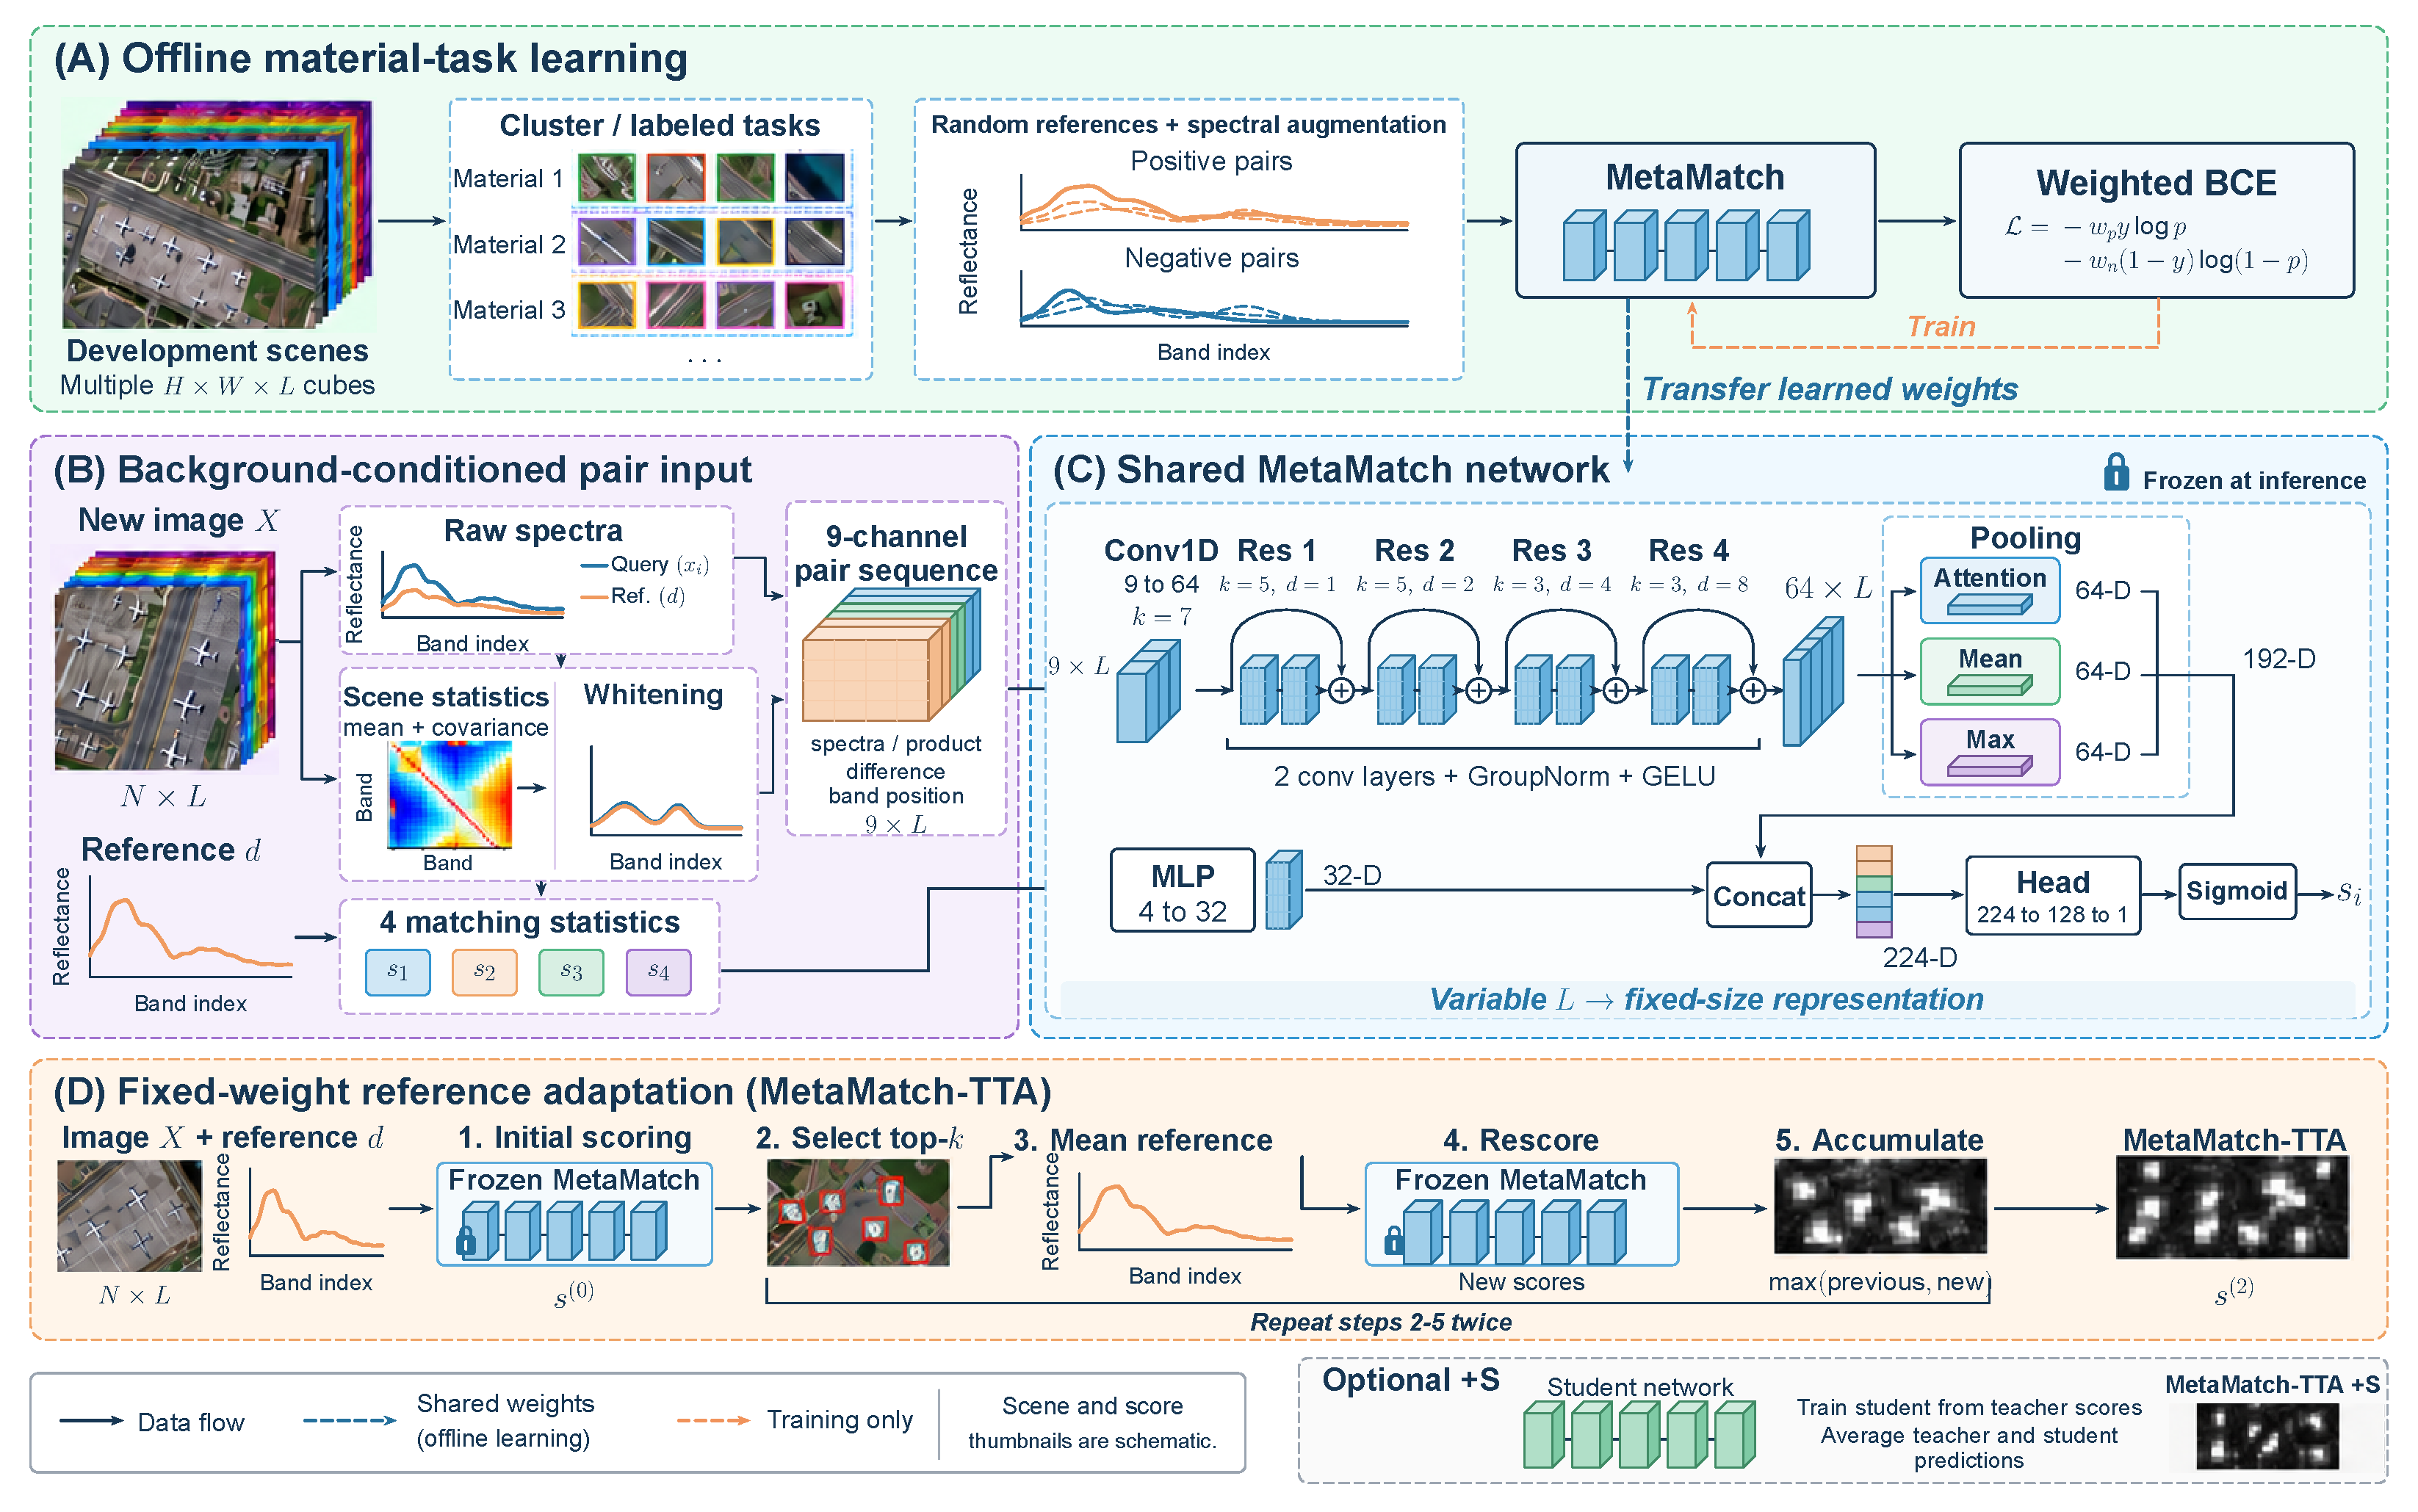
\includegraphics[width=1.0\linewidth]{method_vector/fig_method_vector.pdf}\caption{Architecture and training/inference workflow of \method{}. (A) Material tasks and randomized reference augmentation from development scenes train the shared matcher. (B) Raw spectra, background-whitened spectra, and analytical matching statistics form the paired inputs. (C) Four residual blocks and attention, mean, and maximum pooling extract spectral relationships, which are fused with a statistics branch to predict matching scores. (D) Inference fixes matcher weights and scene statistics while performing two rounds of candidate selection, reference updates, rescoring, and score accumulation. The optional student fusion branch is denoted by \method{} +S and evaluated separately. Scene and response thumbnails are schematic.}\label{full:fig:method}\label{fig:overview}\end{figure}

Fig.~\ref{full:fig:method} organizes cross-material training, background-conditioned inputs, the shared network, and reference adaptation into four connected components. Material tasks and randomized reference augmentation expose the network to different materials and observation conditions. A nine-channel sequence supplies raw and whitened spectral differences and products to a common encoder, while four analytical statistics summarize global matching information. Three pooling operations form a 192-dimensional spectral representation that is combined with a 32-dimensional statistical representation, allowing the prediction head to accommodate different band counts. Inference begins with image-wide scoring, followed by reference updates using the mean of high-scoring candidates and subsequent rescoring. Both rounds reuse the same network and accumulate the pixelwise maximum of previous and new scores. Shared parameters encode material matching knowledge, while background statistics and the reference vector incorporate current-image information, allowing the detector to adapt to new scenes and target references with fixed weights.


\subsection{Background-Conditioned Spectral Representation}
For each image, all spectra and the reference in the same measurement units are scaled by the image-wide maximum. For simplicity, $x_i$ and $d$ below denote the scaled spectra. The mean and covariance over all image pixels are estimated as
\begin{equation}
\mu=\frac{1}{N}\sum_i x_i,\qquad
\widehat\Sigma=\frac{1}{N}\sum_i(x_i-\mu)(x_i-\mu)^\top.
\end{equation}
When targets occupy a small fraction of the image, these statistics mainly reflect background variation, although they are not identical to statistics computed from a true background mask. We apply shrinkage regularization,
\begin{equation}
\Sigma_\gamma=(1-\gamma)\widehat\Sigma+\gamma\frac{\operatorname{tr}(\widehat\Sigma)}{L}I,
\qquad \gamma=0.05,
\end{equation}
and impose an eigenvalue floor of $10^{-10}$ to construct the symmetric whitening matrix $W=\Sigma_\gamma^{-1/2}$. The whitened spectra are then
\begin{equation}
\widetilde x_i=W(x_i-\mu),\qquad \widetilde d=W(d-\mu).
\end{equation}
Whitening rescales directions with large background variability, allowing matching to distinguish deviations that are unusual relative to the current background from proximity in raw spectral values. Retaining the raw branch prevents all discriminative information from depending on covariance estimation.

\subsection{Pair Encoding and Matching Scores}
For each pair $(x_i,d)$, we construct the nine-channel spectral sequence
\begin{equation}
U_i=\left[p,x_i,d,x_i\odot d,x_i-d,
\widetilde x_i,\widetilde d,\widetilde x_i\odot\widetilde d,
\widetilde x_i-\widetilde d\right]\in\R^{9\times L},
\end{equation}
where $p_l=(l-1)/(L-1)$ is the relative band position and $\odot$ denotes elementwise multiplication. Differences and products explicitly describe reference--query relationships, so the network need not infer all pair information from two isolated embeddings.

In addition to the sequence input, the network uses four scalar statistics,
\begin{equation}
v_i=\left[
\frac{\widetilde x_i^\top\widetilde d}{\|\widetilde x_i\|\|\widetilde d\|},\;
\clip\!\left(\frac{\widetilde x_i^\top\widetilde d}{\|\widetilde d\|^2},-3,3\right),\;
\frac{x_i^\top d}{\|x_i\|\|d\|},\;
\log\frac{\|\widetilde x_i\|}{\|\widetilde d\|}
\right].
\end{equation}
A value of $10^{-8}$ is added to each norm for numerical stability. The first two terms are the whitened cosine similarity and a clipped normalized matched-filter projection, respectively. To relate them to AMF~\cite{amf} and ACE~\cite{ace}, let $c_i$ denote the whitened cosine without the numerical stabilization term and $a_i$ the unclipped projection. When the same mean and regularized covariance are used, we obtain
\begin{equation}
\operatorname{ACE}_{\Sigma_\gamma}(x_i,d)=c_i^2,\qquad
\operatorname{AMF}_{\Sigma_\gamma}(x_i,d)=\|\widetilde d\|^2a_i^2.
\end{equation}
The network inputs therefore retain directional and projection information from background-aware matching statistics, while the sequence encoder learns spectral relationships beyond these scalar summaries. These identities explain the analytical origin of the representation. The final detection score is produced by the pair network.

A one-dimensional convolution with kernel size 7 maps the sequence to 64 channels, followed by four residual blocks. Each block contains two convolutions of the same width, GroupNorm with eight groups, and GELU. The four blocks use kernel sizes $(5,5,3,3)$ and dilation rates $(1,2,4,8)$, respectively. Given the output $H_i\in\R^{64\times L}$ and a learnable query $q\in\R^{64}$, we compute
\begin{equation}
a_{il}=\frac{\exp(q^\top H_{il}/\sqrt{64})}{\sum_{j=1}^{L}\exp(q^\top H_{ij}/\sqrt{64})}.
\end{equation}
The attention-weighted mean, ordinary mean, channelwise maximum, and scalar embedding are concatenated to form the prediction-head input,
\begin{equation}
z_i=\left[\sum_l a_{il}H_{il},\ \frac{1}{L}\sum_lH_{il},\ \max_lH_{il},\ \phi(v_i)\right],
\qquad s_i=\sigmoid(g_\theta(z_i)).
\end{equation}
Here, $\phi$ maps the four scalars to 32 dimensions, and $g_\theta$ is a $224\to128\to1$ prediction head with GELU and dropout of 0.1 between the linear layers. The complete model contains 165,857 parameters. Sequence pooling removes the head's dependence on $L$, although relative band positions do not provide physical wavelength calibration across sensors.

\subsection{Material Tasks and Reference Randomization}
Training aims to learn material matching relationships rather than target classes tied to a fixed scene. Each development image is first projected onto at most 30 principal components and partitioned into 40 clusters using $k$-means. Clusters with at least 30 pixels are retained. Each task randomly selects an image and a material cluster and draws 64 positive and 192 negative samples. One quarter of the negatives are drawn from the three other clusters with the nearest whitened centroids, and the remainder from pixels outside the selected material cluster. The clusters provide approximate task labels and are not assumed to correspond to pure physical materials.

Reference construction is randomized across tasks. A single cluster member is selected with probability 0.5, the mean of 2--5 members with probability 0.3, and the mean of the entire cluster with probability 0.2. With probability 0.2, a task instead uses the ground-truth target labels of a development image. In these labeled tasks, targets form the positive class and non-targets form the negative class, without nearest-cluster hard-negative sampling. Training thus uses mixed supervision dominated by clustering tasks, rather than a fully unsupervised or purely self-supervised setting.

References and positive queries are sampled from the same member set. The current implementation does not explicitly exclude the reference pixel from the positive query set. This is consistent with the material-consistency objective, although its effect relative to strictly disjoint reference/query sampling requires separate evaluation. To expose the matcher to reference mismatch, each task augments the reference with probability 0.5 and augments positive and negative query spectra with probabilities 0.6 and 0.3, respectively.

\subsection{Spectral Augmentation and Training Objective}
Spectral augmentation uses the following simplified, physically motivated variation model,
\begin{equation}
\mathcal A(x)=\alpha\big[g(\bm 1+e)\odot x\big]+(1-\alpha)b+\epsilon.
\end{equation}
where $g\sim\mathcal U(0.7,1.3)$ describes a global gain change. The multiplicative variation $e$ is obtained by normalizing a smoothed Gaussian sequence to a standard deviation of 0.08. Mixing is applied with probability 0.5, with $\alpha\sim\mathcal U(0.5,1)$ and background spectrum $b$ sampled from the negative pool of the current task. When mixing is not applied, $\alpha=1$. The additive noise has standard deviation $0.02\bar\sigma_X$, where $\bar\sigma_X$ is the mean of the per-band standard deviations of the image. Whitened spectra are computed after augmentation so that the raw and whitened branches describe the same augmented observation.

Each task contains 256 samples. Training minimizes binary cross-entropy with a positive-class weight of 2,
\begin{equation}
\mathcal L_{\mathrm{task}}=-\frac{1}{256}\sum_i
\left[2y_i\log s_i+(1-y_i)\log(1-s_i)\right].
\end{equation}
Each parameter update accumulates the losses of four tasks. Tasks may have different band counts and are processed in separate forward passes. The model is trained with AdamW for 2,000 steps using a weight decay of $10^{-4}$. The OneCycle schedule has a peak learning rate of $10^{-3}$, with the first 5\% of steps used for warm-up. The gradient norm is clipped at 2. No additional inner loop of parameter adaptation is performed within a task.

\subsection{Reference Refinement with Fixed Weights}
The initial reference $d^{(0)}$ produces scores $s^{(0)}$. We select the highest-scoring $k$ pixels, where
\begin{equation}
k=\clip\big(\lfloor0.002N\rfloor,5,200\big)
\end{equation}
and denote their index set by $\mathcal T^{(r)}$. Their mean spectrum becomes the new reference. At each pixel, we retain the higher response before and after the update,
\begin{align}
d^{(r+1)}&=\frac{1}{k}\sum_{i\in\mathcal T^{(r)}}x_i,\\
\widehat s_i^{(r+1)}&=f_\theta(x_i,d^{(r+1)};\mu,W),\\
s_i^{(r+1)}&=\max\left(s_i^{(r)},\widehat s_i^{(r+1)}\right),\qquad r=0,1.
\end{align}
The two update rounds add two image-wide matching passes. Network parameters and the image whitening statistics remain fixed. The candidate mean estimates a more representative target reference from the current image but does not guarantee the exclusion of incorrect candidates. If the candidate count exceeds the number of true target pixels, the updated reference necessarily includes background. Pixelwise maximization ensures only that individual scores do not decrease, not that target--background ranking improves. We therefore evaluate both $s^{(0)}$ and $s^{(2)}$.

Statistical preprocessing requires approximately $O(NL^2+L^3)$ operations. With a fixed channel width, convolution and pooling costs scale linearly with $NL$, while end-to-end real-time capability depends on measured runtime. The main method does not include a scene-specific student network. Student fusion is evaluated only as an additional control to examine the effect of test-time learning.
\FloatBarrier

\section{Experimental Setup}\label{sec:setup}
\subsection{Data Sources and Scene Splits}
The experiments use six development scenes and six test scenes. Development data support training and method design, while test data are used for detection evaluation. Table~\ref{full:tab:data} records data sources, sensors, spatial dimensions, and mask counts. Fig.~\ref{full:fig:dataset} presents false-color images and ground truth for all twelve scenes.

\begin{table}[H]\centering\scriptsize\setlength{\tabcolsep}{3pt}
\caption{Sensors, locations, dimensions, target pixel counts, and sources of the six test scenes and six development scenes. Dimensions are height $\times$ width $\times$ bands. Files are obtained from public GitHub mirrors or the Wuhan University release.}\label{full:tab:data}
\begin{tabularx}{\linewidth}{l p{2.35cm} l l X l}\toprule
Scene & Sensor, location & Dimensions & Targets & Source & Role \\ \midrule
ABU-A3 & AVIRIS, Los Angeles & $100\times100\times205$ & 170 & \href{https://github.com/sxt1996/Airport-Beach-Urban-ABU}{sxt1996/Airport-Beach-Urban-ABU} & Test \\
ABU-B3 & AVIRIS, Bay Champagne & $100\times100\times188$ & 11 & Same as above & Test \\
ABU-U4 & AVIRIS, Los Angeles & $100\times100\times205$ & 272 & Same as above & Test \\
SanDiego & AVIRIS, San Diego & $100\times100\times189$ & 58 & \href{https://github.com/shendb2022/HTD-Mamba}{shendb2022/HTD-Mamba} & Test \\
HYDICE & HYDICE, urban & $80\times100\times175$ & \shortstack[l]{21\\19 in literature} & \href{https://github.com/sxt1996/HYDICE}{sxt1996/HYDICE} & Test \\
WHR & Headwall Nano, Honghu & $105\times168\times135$ & 36 & \href{http://rsidea.whu.edu.cn}{rsidea.whu.edu.cn} (WHU-Hi-River) & Test \\
\midrule
Segundo & AVIRIS, El Segundo & $250\times300\times224$ & 2048 & \href{https://github.com/sxt1996/Segundo}{sxt1996/Segundo} & Dev. \\
Cri & Nuance CRI & $400\times400\times46$ & 860 & \href{https://github.com/sxt1996/Cri}{sxt1996/Cri} & Dev. \\
ABU-B4 & ROSIS, Pavia & $150\times150\times102$ & 68 & HTD-Mamba & Dev. \\
AVIRIS-2 & AVIRIS, San Diego & $128\times128\times189$ & 120 & \href{https://github.com/sxt1996/AVIRIS-2}{sxt1996/AVIRIS-2} & Dev. \\
SanDiego2 & AVIRIS, San Diego & $100\times100\times189$ & 134 & HTD-Mamba & Dev. \\
ABU-A2 & AVIRIS, airport & $100\times100\times205$ & 87 & HTD-Mamba & Dev. \\
\bottomrule\end{tabularx}\end{table}

Table~\ref{full:tab:data} summarizes the spectral lengths and target sparsity encountered by the shared matcher. Development images contain 46--224 bands, while test images contain 135--205 bands and 11--272 target pixels. Targets account for only 0.11\% of ABU-B3 but 2.72\% of ABU-U4, a roughly 25-fold difference. The evaluation therefore covers both background rejection for sparse targets and identification of more numerous target instances. \method{} reuses the same network under these conditions, and equal scene weighting prevents images with more targets from dominating the aggregate metric. This configuration provides complementary conditions for evaluating the input compatibility of sequence pooling and the cross-image adaptability of background-conditioned matching.

\begin{figure}[H]\centering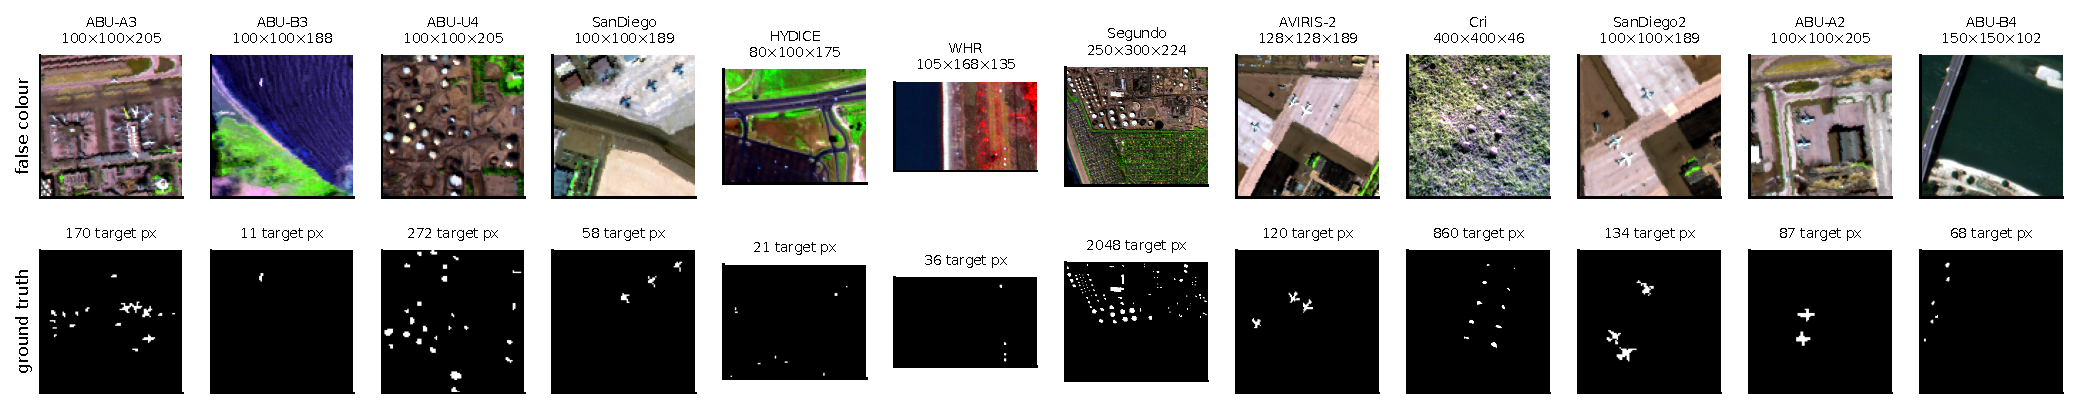
\includegraphics[width=1.0\linewidth]{full_figures/fig_dataset.pdf}\caption{False-color composites and ground-truth masks of the six test scenes (left) and six development scenes (right). Each panel gives image dimensions and target pixel counts. White mask pixels represent the positive class in the evaluated binary detection task.}\label{full:fig:dataset}\end{figure}

Fig.~\ref{full:fig:dataset} shows the scene appearance and target locations in the development and test images. ABU-U4 contains targets in multiple separated regions, whereas positives in ABU-B3 occupy a very small area. A single reference must therefore support both retrieval of same-class instances and rejection of extensive background. \method{} pairs the reference with every query pixel without tying detection to the reference pixel's spatial location, enabling one spectrum to search the whole image. This input organization suits the dispersed target distribution. The single-pixel detection maps and ROC results subsequently evaluate the one-to-many matching capability acquired through material-task learning.

\begin{figure}[H]\centering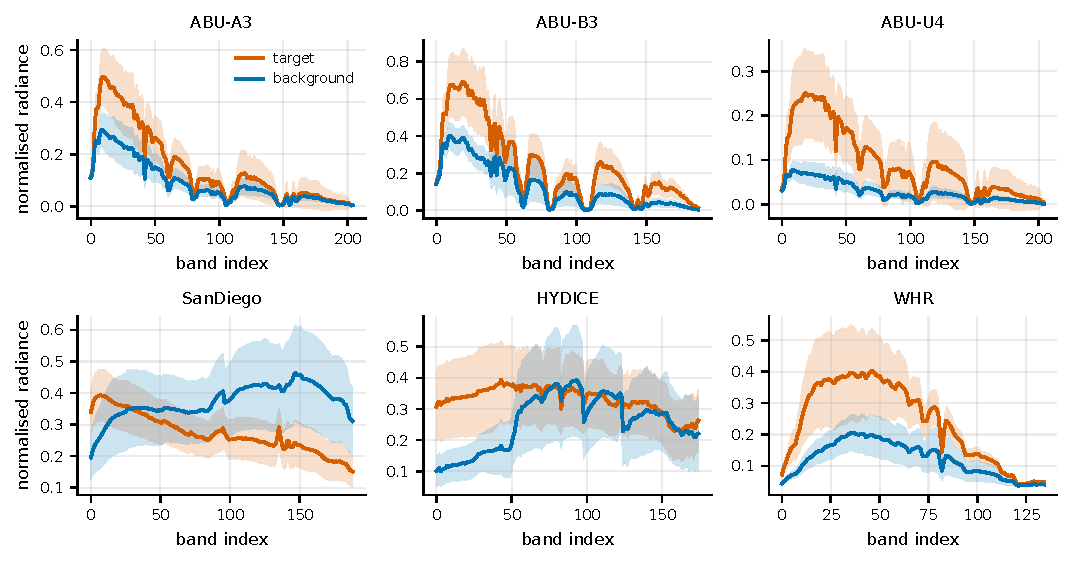
\includegraphics[width=0.85\linewidth]{full_figures/fig_spectra.pdf}\caption{Normalized target and background spectra in the six test scenes. Solid lines indicate means, shaded regions indicate one standard deviation above and below the mean, and the horizontal axis is the band index.}\label{full:fig:spectra}\end{figure}

Fig.~\ref{full:fig:spectra} illustrates the difficulty of identifying targets from raw spectral proximity alone. Targets and background have similar overall shapes in ABU-A3 and ABU-B3, and their distributions overlap in some bands in SanDiego and HYDICE. Within-class variation also allows a single target observation to be far from other target pixels. \matcher{} retains both raw and whitened relationships. The former describes material spectral shape, while the latter reduces the dominance of directions with high background variance, allowing the network to exploit differences that are more discriminative relative to the current background. The figure motivates the paired representation statistically, and the whitening ablation in Table~\ref{full:tab:devab} evaluates the benefit of background conditioning through detection accuracy.


WHR uses the anomaly-detection mask in the public release, with 36 positive pixels. The local public HYDICE mask contains 21 positive pixels, compared with 19 in the comparison paper. These masks define the current binary detection tasks and are not equivalent to material classes verified by compositional analysis. AVIRIS-1 shares the SanDiego image but has different annotations and is excluded from the development pool. Exact matching of raw float32 spectra across four development/test image pairs with equal band counts found no identical spectral records. Some scenes share sensor sources, so the experiments evaluate transfer to new images rather than strict generalization to unseen sensors.

Development evaluation uses two complementary splits. Split A trains on AVIRIS-2, SanDiego2, and ABU-A2 and evaluates on Segundo, Cri, and ABU-B4. Split B exchanges the roles of these groups. Component ablations use split A with complete records and training seed 0. Final models are trained on all six development scenes using seeds 0, 1, and 2. Cluster tasks and labeled target tasks, selected with probability 0.2, are jointly used. The model therefore receives target supervision from the development scenes.

\subsection{Reference Spectrum Protocols}
The following protocols separately examine reference information and mismatch.
\begin{itemize}
\item \textbf{P0: Ground-truth mean reference.} The mean spectrum of all ground-truth target pixels in the test image provides an information-rich reference condition. It uses the complete target region rather than a single independent reference measurement.
\item \textbf{P1: Single-pixel reference.} One ground-truth target pixel is randomly selected from the test image to evaluate the representativeness of a single observation. This is a same-image reference, and the sampled pixel is not removed from the evaluation mask.
\item \textbf{P2: Few-pixel mean reference.} The mean of $k=3$ or $5$ randomly selected target pixels evaluates the effect of the reference sample count.
\item \textbf{P4: Perturbed reference.} The P0 reference is modified by a gain in $[0.7,1.3]$, smooth multiplicative variation with standard deviation 0.08, and additive noise. The noise standard deviation is 2\% of the across-band standard deviation of the transformed reference. This is a synthetic stress test using ground-truth information, not an external spectral measurement.
\item \textbf{P3: Cross-image reference.} The target mean from another image with the same band layout is used as the reference, with brightness scaling adjusted according to the source and test-image maxima. The image pairs are listed in Table~\ref{full:tab:p3}. They evaluate cross-image reference transfer, but the available records have not verified that donor and test targets have exactly the same physical material identity.
\end{itemize}

\begin{figure}[H]\centering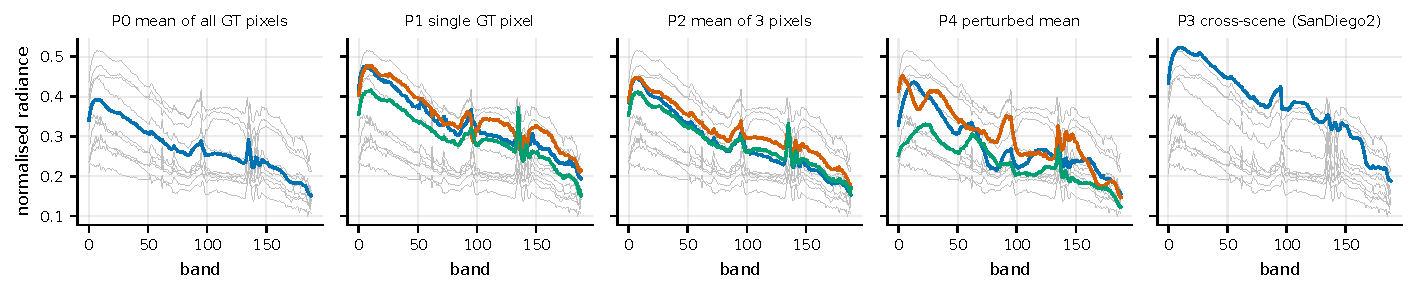
\includegraphics[width=1.0\linewidth]{full_figures/fig_protocols.pdf}\caption{Reference spectrum construction for SanDiego. Gray curves are ground-truth target spectra. The panels show the P0 mean, three P1 single-pixel references, three P2 three-pixel means, three P4 perturbed references, and the P3 reference from SanDiego2. The vertical axis is normalized spectral intensity.}\label{full:fig:protocols}\end{figure}

Fig.~\ref{full:fig:protocols} illustrates input variation for the same target under different reference constructions. A P1 observation retains within-target variation, a P2 mean reduces the influence of individual observations, P4 changes gain, shape, and noise around the mean, and P3 moves the reference source to another image. \method{} uses the same pair interface for all these references. Reference budget and imaging variation are expressed through the inputs, with the architecture and weights held constant. Performance changes across protocols therefore reveal the response of the shared matcher to changes in target description and provide controlled comparisons for analyzing reference randomization and spectral augmentation.

\subsection{Comparison Methods and Implementation Settings}
The main comparisons with recent methods include SPWCG-HTD~\cite{spwcg2026} and the RS-MF family~\cite{rsmf2026}. Published AdvGMM + FAME-Net~\cite{fame} results are additionally included for mean references. Literature values are taken directly from the experimental tables of the original papers, whereas \matcher{} and \method{} use our recorded experiments. FAME-Net uses a target mean reference. SPWCG-HTD selects the pixel closest to the mean of all target pixels. The RS-MF family uses the mean of a small set of labeled target pixels without specifying the exact sample count. Representative-pixel selection and random single-pixel references are identified separately, and few-pixel means are reported under their recorded sampling settings.

Reference information and output stages are evaluated through internal controls of our model. Complete per-scene results are provided in Supplementary Section~\ref{app:protocol_detail}. Section~\ref{sec:recent} examines comparisons under limited reference information.

SPWCG-HTD~\cite{spwcg2026} selects pseudo-targets in the current scene and trains its detector through diffusion-based generation and contrastive learning. RS-MF and Adaptive RS-MF~\cite{rsmf2026} produce scores through subspace background statistics and filter ensembles. The latter perturbs the reference and selects ensemble members. Our material matcher is trained on development scenes, with network weights held fixed at test time. Table~\ref{full:tab:params} summarizes model configurations and new-scene processing for the methods in the main comparisons.

\begin{table}[H]\centering\small\setlength{\tabcolsep}{5pt}\renewcommand{\arraystretch}{1.15}
\caption{Model configurations and new-scene processing for the methods in the main comparisons. Literature configurations follow the original method and implementation sections. Our configurations correspond to the implemented network.}\label{full:tab:params}
\begin{tabularx}{\linewidth}{l X p{0.23\linewidth}}\toprule
Method & Detection configuration & Network-weight optimization on a new scene \\ \midrule
SPWCG-HTD (2026)~\cite{spwcg2026} & Wavelet cross-gating, convolution kernel and stride of 9, 128-dimensional Transformer with 2 layers and 4 heads & Train the diffusion generator and detection encoder \\
RS-MF (2026)~\cite{rsmf2026} & 50 random subspaces with 30 bands each & No gradient training, analytical filter solution \\
Adaptive RS-MF (2026)~\cite{rsmf2026} & Same subspaces, reference perturbation coefficient 0.01, response-contrast selection and weighted fusion & No gradient training, analytical filter solution \\
\matcher{} & 9-channel paired input, 64 channels, 4 residual blocks, one image-wide scoring pass & Fixed development-stage weights \\
\method{} & Same network as \matcher{}, two reference updates, three image-wide scoring passes in total & Fixed development-stage weights \\
\bottomrule\end{tabularx}
\end{table}

Table~\ref{full:tab:params} shows how the methods establish detection rules for a new image. The RS-MF family analytically derives filters from background statistics, while SPWCG-HTD learns representations through sample generation and encoder training in the current scene. \method{} concentrates material relation learning in the development stage. A new image updates only the background conditions and reference input. Both reference-update rounds reuse the same weights and background-whitening results. Scene adaptation therefore adds no network parameters and avoids scene-specific gradient optimization, illustrating the separation between shared matching and adaptation through the inputs.


\subsection{Evaluation Metrics and Statistical Aggregation}
ROC-AUC is the primary discrimination metric. We also retain the five measures used in three-dimensional ROC analysis~\cite{chang2021}. For normalized detection scores and threshold $\tau$, let $P_D(\tau)$ and $P_F(\tau)$ denote detection and false-alarm probabilities, respectively. We define
\begin{align}
\mathrm{AUC}_1&=\int_0^1P_D(P_F)\,\mathrm dP_F,\\
\mathrm{AUC}_2&=\int_0^1P_F(\tau)\,\mathrm d\tau,\qquad
\mathrm{AUC}_3=\int_0^1P_D(\tau)\,\mathrm d\tau,\\
\mathrm{AUC}_4&=\mathrm{AUC}_1+\mathrm{AUC}_3-\mathrm{AUC}_2,\qquad
\mathrm{AUC}_5=\mathrm{AUC}_3/\mathrm{AUC}_2.
\end{align}
AUC$_1$ measures target--background ranking over the full threshold range. AUC$_2$ measures the integrated false-alarm response, with a smaller value indicating stronger background suppression. Larger values are preferred for the other metrics. Each detection map is min--max normalized before integration over all unique thresholds. Strictly increasing transformations preserve ROC-AUC but can change threshold-integral metrics. AUC$_5$ can become very large when the false-alarm integral approaches zero and should therefore be interpreted together with the other measures.

P1, P2, and P4 share reference draw indices 0, 1, and 2, with generation seeds $1000+\mathrm{draw}$. For our models, the three reference draws are averaged within each training seed, followed by an equally weighted average over the three seeds. Recent comparison methods use published values and are not included in our training-seed statistics. P0 and P3 have one reference per scene and seed. Reported standard deviations describe variation over the corresponding runs, including training and reference variation where applicable. They are not confidence intervals over independent scenes.

Macro-averages weight scenes equally. P3 contains three image pairs, whereas the other test protocols contain six scenes. Values are reported to four decimal places, with the best values in each comparison group in bold. Ties at the displayed precision are marked jointly. The minimum is preferred for AUC$_2$. Results for individual training seeds are given in Table~\ref{tab:seeds}.

\subsection{Output Stages and Computing Environment}
\matcher{} denotes direct pair matching, and \method{} denotes the output after two gradient-free reference refinements. The student fusion configuration, \method{} +S, is the equally weighted average of the refined teacher and an optional student. Student training settings are provided in the supplementary material. The main quantitative results use the refined matcher. Stored detection maps contain the +S output, so ROC curves, detection maps, and score distributions explicitly identify that configuration. Experiments were conducted on a shared NVIDIA GB10 system with 128 GB of unified memory.
\FloatBarrier

\section{Experimental Results and Analysis}\label{sec:results}
This section examines the performance of \method{} and the sources of its gains through comparisons with recent methods, component ablations, changes in reference information, and comparisons of output stages. We investigate whether the shared matcher reduces dependence on a complete target reference, how background conditioning and spectral augmentation improve discrimination, and how scene candidates supplement the reference while network weights remain fixed. ROC curves, spatial responses, and score distributions are then used to relate target detection to background suppression. Each analysis connects observed performance to the corresponding design and its practical role.

\subsection{Comparison with Recent Methods}\label{sec:recent}
We compare \method{} with recent methods under random single-pixel and five-pixel mean references, using ROC-AUC to evaluate the ability of previously learned material relationships to support detection in new images.

\begin{table}[H]\centering\small\setlength{\tabcolsep}{7pt}
\caption{ROC-AUC on SanDiego with a single-pixel reference. SPWCG-HTD results are taken from Table 3 of the original paper. Our P1 results aggregate three training seeds. $\Delta$ denotes the difference from the published SPWCG-HTD value in percentage points. The highest ROC-AUC is bold.}\label{tab:selected_single}
\begin{tabular}{llcc}\toprule
Method & Reference selection & ROC-AUC $\uparrow$ & $\Delta$ \\ \midrule
SPWCG-HTD (2026)~\cite{spwcg2026} & Representative pixel & 0.96855 & -- \\
\matcher{} & Random single pixel & 0.9912 & +2.27 \\
\method{} & Random single pixel & \textbf{0.9914} & +2.29 \\
\bottomrule\end{tabular}
\par\vspace{3pt}\begin{minipage}{0.98\linewidth}\footnotesize
The published method selects the pixel closest to the mean of all targets. Its San Diego A image contains $100\times100\times224$ samples and 57 target pixels, whereas ours contains $100\times100\times189$ samples and 58 target pixels. The published standard deviation over three seeds is 0.03467. Differences describe the numerical relationship between results reported across studies.
\end{minipage}\end{table}

Table~\ref{tab:selected_single} compares detection on SanDiego with a single-pixel input. \method{} achieves a ROC-AUC of 0.9914, exceeding the published SPWCG-HTD value by 2.29 percentage points. Our reference is sampled randomly from the target set, and performance remains high when aggregated over three reference draws and three training seeds. Thus, the model can use an ordinary individual target observation to retrieve targets throughout the image. Direct \matcher{} already achieves 0.9912, indicating that the underlying discrimination is acquired through pairwise learning during development. This result supports organizing different materials and their observation variations into training tasks so that shared matching rules reduce dependence on reference representativeness and retraining within a new scene.

\begin{table}[H]\centering\small\setlength{\tabcolsep}{10pt}
\caption{ROC-AUC on ABU-A3 with a few-pixel reference. RS-MF and Adaptive RS-MF results are taken from Table 1 of the original paper. Our results use the five-pixel mean reference in P2 and aggregate three training seeds. The highest ROC-AUC is bold.}\label{tab:selected_few}
\begin{tabular}{llc}\toprule
Method & Number of reference pixels & ROC-AUC $\uparrow$ \\ \midrule
RS-MF (2026)~\cite{rsmf2026} & -- & 0.976 \\
Adaptive RS-MF (2026)~\cite{rsmf2026} & -- & 0.978 \\
\matcher{} & $k=5$ & \textbf{0.9812} \\
\method{} & $k=5$ & 0.9797 \\
\bottomrule\end{tabular}
\par\vspace{3pt}\begin{minipage}{0.98\linewidth}\footnotesize
``--'' indicates that the reference pixel count is unspecified in the original paper, which constructs the reference from the mean of a small set of labeled targets. The spatial dimensions and band count of ABU-A3 agree across the studies. Pixelwise mask agreement has not been verified.
\end{minipage}\end{table}

Table~\ref{tab:selected_few} evaluates detection when the reference is formed from a few target observations. \method{} achieves 0.9797 on ABU-A3, exceeding the published RS-MF and Adaptive RS-MF values by approximately 0.37 and 0.17 percentage points, respectively. Direct \matcher{} achieves 0.9812, showing that the pairwise network can distinguish targets from background using a five-pixel mean before reference refinement. Relative to the three-pixel reference in the same scene, direct matching and reference refinement improve by 1.15 and 1.32 percentage points, respectively. Additional observations can therefore improve ranking directly through the reference input. This result demonstrates the ability of the shared matching function to exploit different reference budgets and supports reference randomization as a way to learn a unified detection interface.

\subsection{Material Tasks and Component Analysis}
The component analysis controls the training split, budget, and reference draws while removing either spectral augmentation or the whitened sequence channels. It tests whether these designs improve material discrimination in scenes excluded from training. Results after reference refinement evaluate the complete pipeline, whereas ablations of direct matching identify whether gains emerge before candidate updates. Together, these experiments distinguish the contribution of the pairwise representation from changes induced by reference refinement.


\begin{table}[H]\centering\footnotesize\setlength{\tabcolsep}{4pt}\renewcommand{\arraystretch}{1.12}
\caption{Component ablations of \textbf{\method{}} on development split A. Each entry reports AUC$_1\uparrow$ / AUC$_2\downarrow$ after reference refinement. Each metric is compared separately within a row, with the best value in bold. All configurations use training seed 0. Scalar side information is retained when the whitened sequence channels are removed.}\label{full:tab:devab}
\begin{lrbox}{\fulltablebox}\begin{tabular}{lcccc}\toprule
Protocol & Scene & \textbf{\method{}} & w/o augmentation & w/o whitened channels \\ \midrule
P0 & Segundo & \textbf{0.9938} / 0.010 & 0.9842 / \textbf{0.005} & 0.9908 / 0.049 \\
 & Cri & \textbf{0.9995} / 0.131 & 0.9216 / \textbf{0.057} & 0.9718 / 0.564 \\
 & ABU-B4 & \textbf{0.9339} / 0.021 & 0.8982 / \textbf{0.010} & 0.8877 / 0.152 \\
P1 & Segundo & 0.9822 / 0.023 & \textbf{0.9870} / \textbf{0.007} & 0.9841 / 0.049 \\
 & Cri & \textbf{0.9994} / 0.128 & 0.9215 / \textbf{0.065} & 0.9802 / 0.555 \\
 & ABU-B4 & \textbf{0.9168} / 0.047 & 0.8926 / \textbf{0.016} & 0.8217 / 0.140 \\
P2 ($k=3$) & Segundo & \textbf{0.9887} / 0.018 & 0.9872 / \textbf{0.005} & 0.9821 / 0.059 \\
 & Cri & \textbf{0.9995} / 0.120 & 0.8986 / \textbf{0.053} & 0.9570 / 0.539 \\
 & ABU-B4 & \textbf{0.9303} / 0.045 & 0.8952 / \textbf{0.019} & 0.8656 / 0.148 \\
P4 & Segundo & \textbf{0.9922} / 0.021 & 0.9910 / \textbf{0.012} & 0.9904 / 0.037 \\
 & Cri & \textbf{0.9996} / 0.172 & 0.9522 / \textbf{0.061} & 0.9732 / 0.587 \\
 & ABU-B4 & \textbf{0.9322} / 0.036 & 0.9200 / \textbf{0.020} & 0.8930 / 0.125 \\
\bottomrule\end{tabular}\end{lrbox}\ifdim\wd\fulltablebox>\linewidth\resizebox{\linewidth}{!}{\usebox{\fulltablebox}}\else\usebox{\fulltablebox}\fi\end{table}

In Table~\ref{full:tab:devab}, the complete \method{} obtains the highest ROC-AUC in 11 of the 12 scene--protocol combinations. Its P1 accuracy on Cri is 0.9994, exceeding the value without augmentation, 0.9215, by 7.79 percentage points. On ABU-B4, the complete model achieves 0.9168, improving by 2.42 and 9.51 percentage points over the configurations without augmentation and without whitened channels, respectively. Although all references contain only one pixel, the complete model ranks targets more accurately, attributing the gains to how training and representation handle limited reference information. Spectral augmentation requires the model to recognize the same material despite changes in gain and spectral shape. The whitened sequences describe the reference and query relative to the current background. These comparisons support the roles of augmentation in tolerating observation changes and background conditioning in distinguishing spectrally similar land-cover materials.



For these two scenes, gains also appear in the direct-matching results in Supplementary Table~\ref{tab:ablation}, indicating that the components improve discrimination before candidates are generated. On ABU-B4 under P1, the complete model reduces AUC$_2$ from 0.140 without whitened channels to 0.047 while increasing ROC-AUC, combining improved ranking with a lower integrated background response. The configuration without augmentation has a lower AUC$_2$ but also a lower ROC-AUC. Compressing scores alone therefore does not imply better target discrimination. On Segundo under P1, the complete model, the configuration without augmentation, and the configuration without whitened channels achieve 0.9822, 0.9870, and 0.9841, respectively, showing that component gains vary across tasks. Taken together, ranking, response, and output-stage evidence demonstrate measurable discrimination gains from spectral variation training and background-conditioned representation on Cri and ABU-B4.

\subsection{Detection under Changes in Reference Information}
\begin{table}[H]\centering\small\setlength{\tabcolsep}{7pt}
\caption{Macro-average ROC-AUC of \matcher{} and \method{} under the reference protocols. P3 contains three image pairs, and the other protocols contain six target scenes. The higher value in each row is bold.}\label{tab:reference_profile}
\begin{tabular}{llcc}\toprule
Protocol & Reference construction & \matcher{} & \method{} \\ \midrule
P0 & Mean of all targets & \textbf{0.9925} & 0.9924 \\
P1 & Random single pixel & 0.9895 & \textbf{0.9902} \\
P2 ($k=3$) & Three-pixel mean & \textbf{0.9900} & 0.9899 \\
P2 ($k=5$) & Five-pixel mean & 0.9922 & \textbf{0.9924} \\
P4 & Synthetically perturbed reference & \textbf{0.9914} & 0.9903 \\
P3 & Cross-image reference & \textbf{0.9891} & 0.9874 \\
\bottomrule\end{tabular}
\end{table}

Table~\ref{tab:reference_profile} compares the effects of reference information and reference variation on the same network with fixed weights. \method{} achieves 0.9902 with a random single-pixel reference, only 0.22 percentage points below the 0.9924 obtained with the complete target mean. The five-pixel mean also achieves 0.9924, matching the complete mean at the reported precision of four decimal places. High detection accuracy therefore does not require collecting all target pixels to estimate a reference. A few observations can already invoke the material relationships learned during development. The three-pixel result of 0.9899 is close to the single-pixel result, indicating that reference quality also depends on the target variations covered by sampling, rather than sample count alone. For detection with limited reference information, these results show that near-full-reference ranking accuracy can be maintained with much less target information. They support training a shared matcher jointly through material tasks and reference randomization.

With synthetically perturbed references, direct \matcher{} achieves 0.9914, only 0.11 percentage points below its P0 value of 0.9925. The model handles the prescribed gain changes, smooth deformations, and noise before reference refinement, indicating that this tolerance is embedded in the learned matching function. \method{} maintains 0.9903 under P4 and achieves 0.9874 over three exploratory cross-image pairs, demonstrating the use of the fixed-weight interface as references change. P4 uses synthetic variation families that overlap with the training augmentations, whereas P3 uses three pairs with compatible band layouts. Alongside the ablations, these results support incorporating reference insufficiency and spectral variation into development-stage learning to reduce the need to refit a detector for a new scene.

\subsection{Roles of Matching, Reference Refinement, and Student Fusion}
\begin{figure}[H]\centering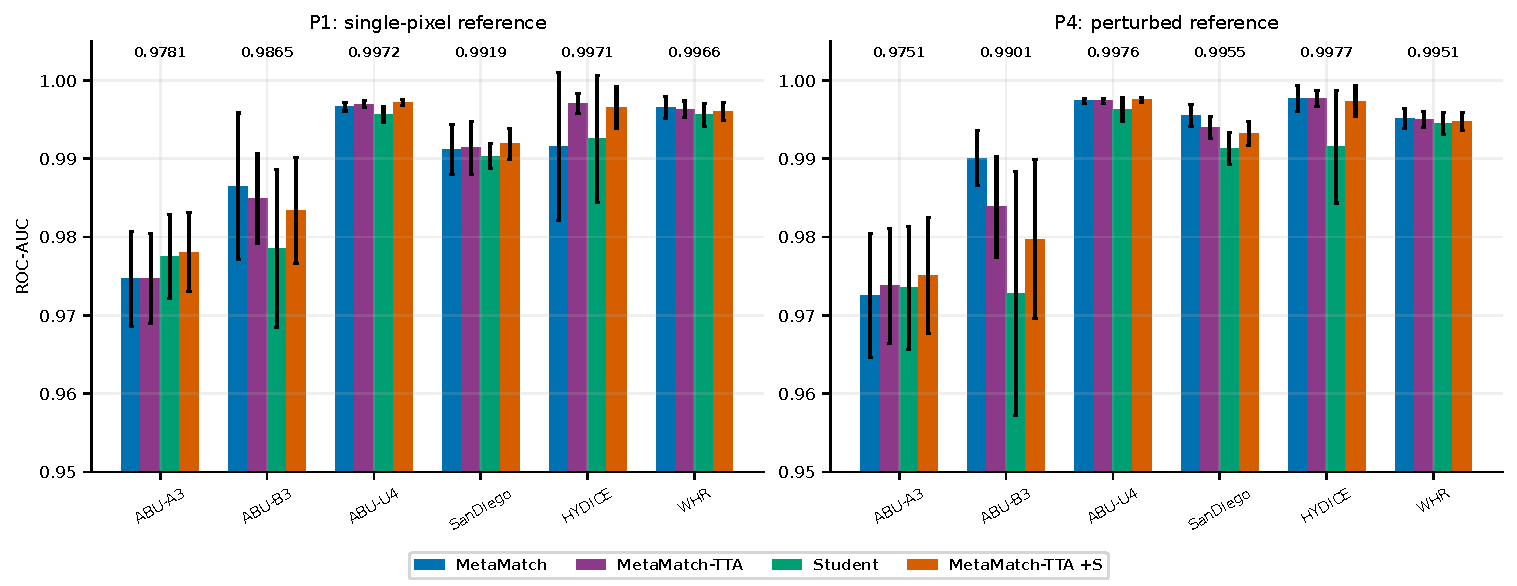
\includegraphics[width=1.0\linewidth]{recent_only_figures/fig_targets_stages.pdf}\caption{Output-stage comparison under P1 and P4, evaluating \matcher{}, \method{}, the student, and the teacher--student mean separately. Error bars show descriptive standard deviations over three reference draws and three training seeds. The highest scene mean is bold. Both panels display the vertical range 0.95--1.005.}\label{full:fig:stages}\end{figure}

Figure~\ref{full:fig:stages} separates the contributions of shared matching, reference updates, and student fusion through scene-specific outputs. Their macro-average ROC-AUC values under P1 are 0.9895, 0.9902, and 0.9905, respectively. Direct matching already provides strong discrimination. Reference updates improve performance by approximately 0.07 percentage points without adding learnable parameters, and student fusion adds approximately 0.03 percentage points. These increments show that supplementing the reference with information from the current image is an effective form of adaptation. Most detection capability can be obtained while retaining fixed network weights. The stage comparison thus supports combining reusable matching rules with reference-vector updates to exploit both knowledge learned across scenes and information in the current image.

Under P4, the three stages achieve 0.9914, 0.9903, and 0.9896, respectively, with direct matching obtaining the highest macro-average accuracy. Compared with P1, the initial P4 reference is derived from the mean of all targets and retains more complete target information. Its main change is the prescribed spectral perturbation. Since the shared matcher already tolerates these variations, incorporating image candidates does not necessarily provide a better target description. This comparison distinguishes the roles of the two designs. Spectral variation training establishes discrimination under reference mismatch, while reference updates supplement scene evidence when an individual observation is insufficient.

Figure~\ref{fig:refine} evaluates reference updates using paired differences within the same runs. Under P1, the ROC-AUC on HYDICE increases from 0.9916 to 0.9971, a gain of approximately 0.55 percentage points, while the corresponding standard deviation decreases from 0.0095 to 0.0013. Higher average accuracy and reduced variability occur together, indicating that references formed from high-scoring candidates reduce sensitivity to the initial single-pixel choice in this scene. The update aggregates candidate observations dispersed throughout the image into the reference without retraining the network, giving the existing matching rules a more complete target description. Both accuracy and stability across runs support the ability of gradient-free reference updates to compensate for insufficient information in a single observation.

\begin{figure}[htbp]\centering
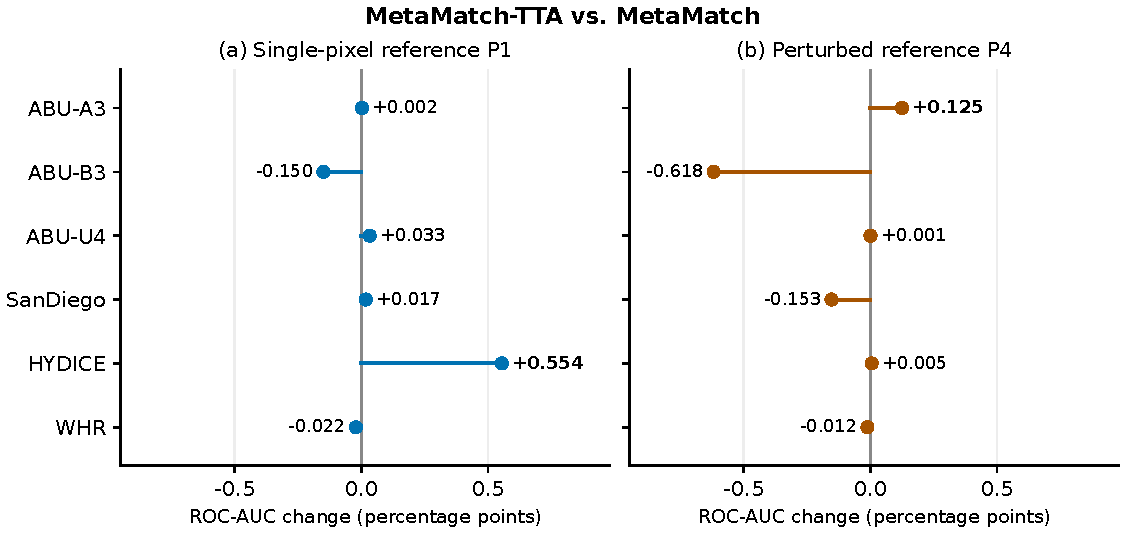
\includegraphics[width=.98\linewidth]{english_figures/refinement_effect.pdf}
\caption{Scene-specific ROC-AUC changes of \textbf{\method{}} relative to \textbf{\matcher{}}. Each point is the mean paired difference over three reference draws and three training seeds. Values are in AUC percentage points, with the largest gain within each protocol in bold. Values to the right of zero indicate improvement.}\label{fig:refine}
\end{figure}

The P1 result changes from 0.9865 to 0.9850 on ABU-B3 and from 0.9966 to 0.9963 on WHR, indicating that the quality of the reference mean also depends on candidate composition. ABU-B3 contains only 11 ground-truth target pixels, but the update selects 20 candidates. Even if all targets are selected, at least nine nontarget pixels contribute to the mean. Thus, a fixed candidate count introduces background components when targets are extremely sparse, making material consistency central to reference supplementation. The gain on HYDICE and this sparse-target comparison show that the matcher supplies the basis for candidate discrimination, while candidate selection determines the quality of the added information. The reference vector becomes an explicit object for analyzing and improving adaptation while shared network weights remain unchanged.

The student-fusion comparison evaluates whether shared matching scores can support additional learning within the scene. Under P1, \method{} and the fused output achieve 0.9902 and 0.9905, respectively, indicating that teacher scores can support a complementary student branch. Under P4, their results are 0.9903 and 0.9896, showing that extra fitting does not improve ranking under every reference condition. We evaluate the student as a separate extension and retain shared matching and gradient-free reference updates as the main method. Consequently, the main pipeline already approaches the fused P1 accuracy without training a scene-specific student. This comparison supports using reference adaptation for the principal online adjustment and reducing dependence on test-time network optimization.
\FloatBarrier

\subsection{ROC Curves, Spatial Responses, and Score Distributions}
\begin{figure}[H]\centering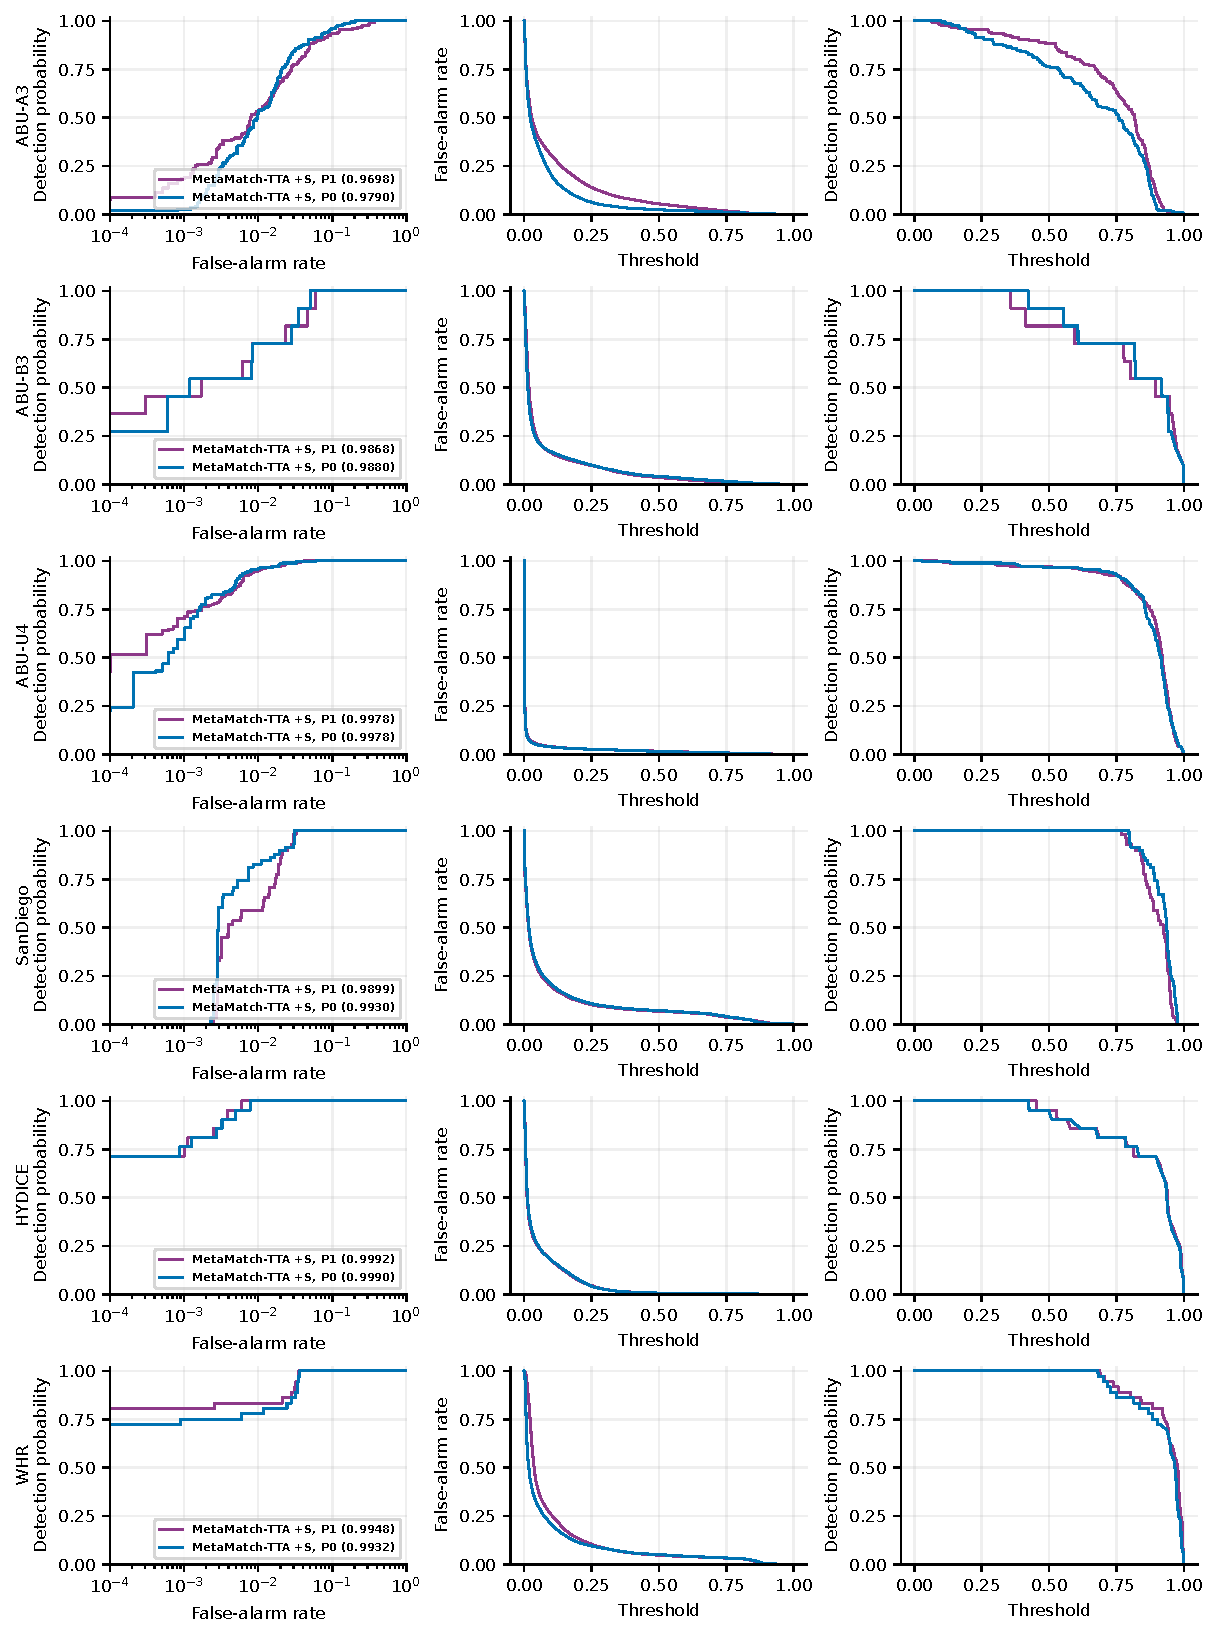
\includegraphics[width=.97\linewidth,height=.62\textheight,keepaspectratio]{recent_only_figures/fig_roc.pdf}\caption{ROC analysis of \method{} +S under P1 and P0. Training seed 0 is used, with reference draw 0 for P1. Columns show detection probability versus false-alarm rate, false-alarm rate versus normalized threshold, and detection probability versus normalized threshold, respectively. Legends report the ROC-AUC of each detection map.}\label{full:fig:roc}\end{figure}

Figure~\ref{full:fig:roc} examines single-reference discrimination by \method{} +S through the relationship between target detection and background false alarms. The plotted results use training seed 0 and reference draw 0 for P1. Quantitative tables summarize repeated runs. On ABU-U4, the P1 and P0 ROC-AUC values both equal 0.9978 at four decimal places, and the curves remain close over much of the false-alarm range. A reference formed from one target pixel therefore retains ranking information close to that provided by the complete target mean. From the detection scores corresponding to this figure, P1 detection rates at a false-alarm rate no greater than 1\% are 95.22\% on ABU-U4 and 100\% on HYDICE. A single reference thus enables the detection of most targets in these images while limiting background false alarms, rather than merely assigning high scores to a few targets. This threshold-based evidence supports the ability of material-task learning to generalize an individual observation to other target instances.

The final two columns explain how this ranking emerges. On ABU-U4, the background response falls rapidly as the threshold increases, while the target response remains high over a broad threshold interval. Target enhancement and background suppression jointly create a useful discrimination interval. The background response on ABU-A3 decays more slowly, consistent with its P1 ROC-AUC of 0.9698. The high-score tail of similar background materials still affects detection at strict thresholds. This analysis identifies the intended role of background-conditioned representation in separating target similarity from background similarity in the current scene. Together with the whitening ablation, the curves support incorporating scene statistics into material pairing to improve relative discrimination.

\begin{figure}[H]\centering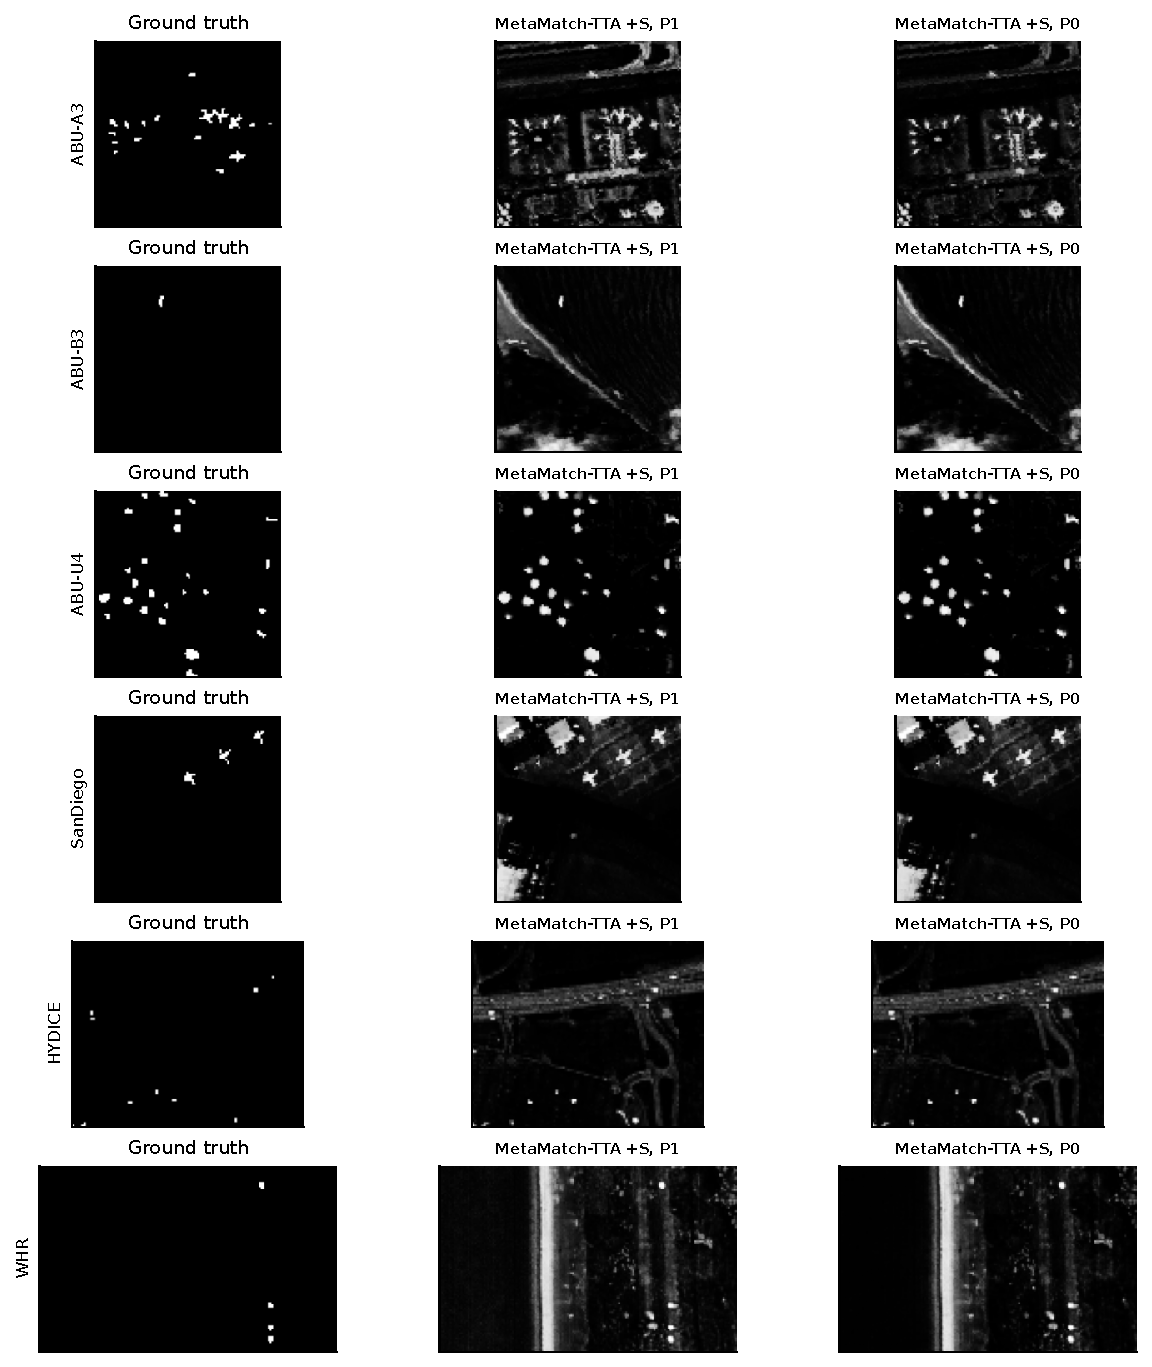
\includegraphics[width=1.0\linewidth,height=.68\textheight,keepaspectratio]{recent_only_figures/fig_maps.pdf}\caption{Spatial detection results of \method{} +S. Columns show ground truth, P1 single-pixel-reference output, and P0 mean-reference output, respectively. All results use training seed 0, with reference draw 0 for P1. Each detection map is independently min--max normalized, and brighter pixels indicate higher scores.}\label{full:fig:maps}\end{figure}

Figure~\ref{full:fig:maps} compares ground-truth locations, single-pixel-reference outputs, and complete-mean-reference outputs to determine whether high ROC-AUC corresponds to responses in actual target regions. Because each map is independently normalized, the analysis uses target locations and within-map contrast. On ABU-U4, the P1 output exhibits bright responses at multiple separated targets while most surrounding background remains low, yielding a ROC-AUC of 0.9978. On HYDICE, dispersed small targets also receive strong P1 responses, with a ROC-AUC of 0.9992. Although the model receives only one reference spectrum, it identifies similar materials elsewhere in the image. These results illustrate the coverage of multiple target instances provided by pairwise task learning.

The P1 and P0 outputs on ABU-U4 and HYDICE exhibit similar spatial target distributions, indicating that fewer reference observations do not confine the response to a single instance. ABU-A3, SanDiego, and WHR also retain responses to some background structures, so the spatial outputs should be interpreted alongside false-alarm behavior in the ROC curves. Pixelwise spectral pairing produces these target responses without requiring target coordinates as input, demonstrating the role of reference--query modeling in image-wide material retrieval. These visualizations provide spatial evidence for one-to-many detection from a single reference and complement the adaptability observed with randomized-reference training.

\begin{figure}[H]\centering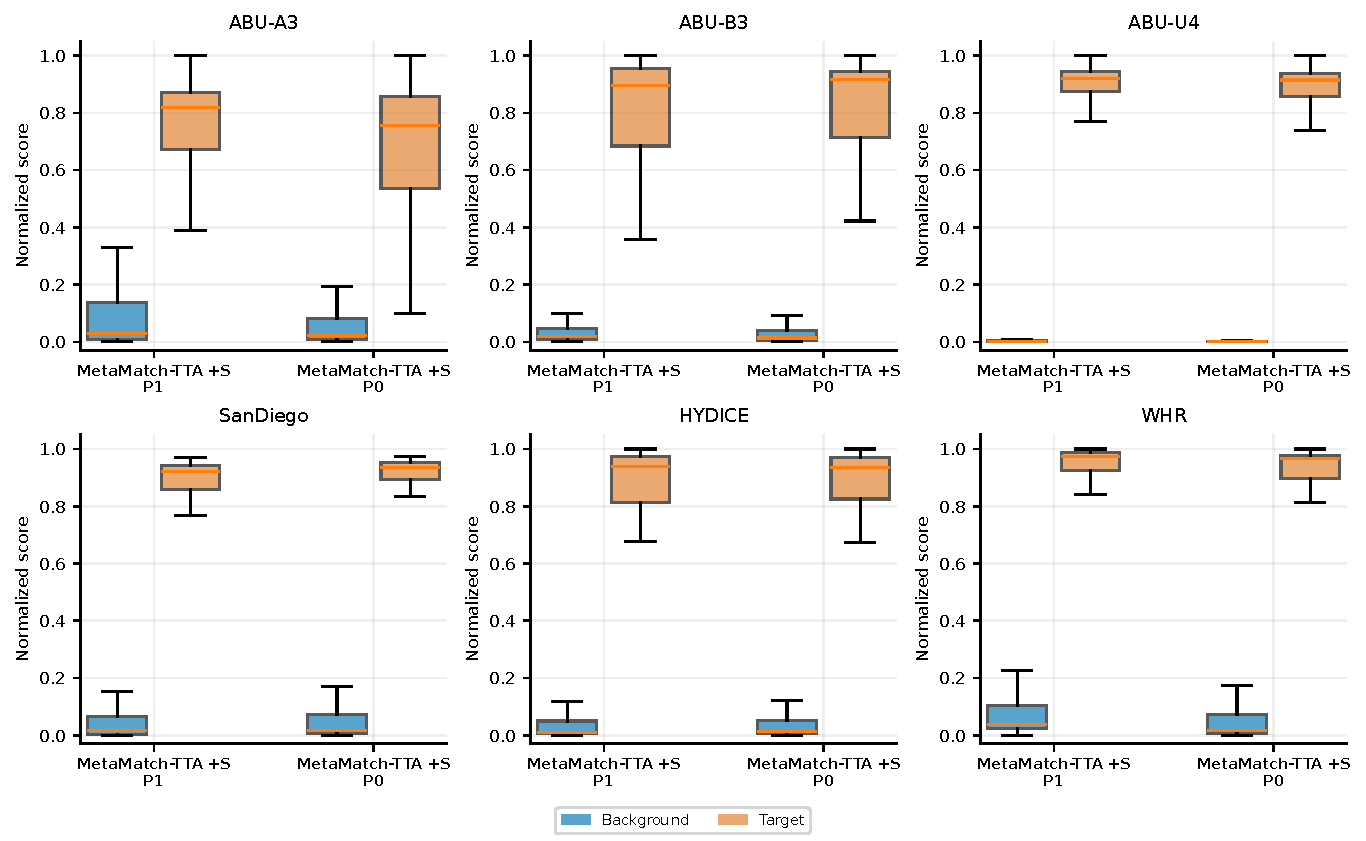
\includegraphics[width=1.0\linewidth]{recent_only_figures/fig_box.pdf}\caption{Background and target score distributions of \method{} +S under P1 and P0, using the same detection maps as Fig.~\ref{full:fig:maps}. Blue denotes background and orange denotes targets. Boxes indicate interquartile ranges, horizontal lines indicate medians, and outliers are omitted.}\label{full:fig:box}\end{figure}

Figure~\ref{full:fig:box} explains the target ranking of \method{} +S through the central portions of pixel-score distributions. Target and background interquartile ranges are separated under both P1 and P0 in all six scenes, providing distributional evidence for the high detection accuracy. On ABU-U4 under P1, the lower quartile of target scores is 0.8740, whereas the upper quartile of background scores is only 0.0028. The corresponding values on HYDICE are 0.8135 and 0.0497. Most targets therefore maintain high responses while most background pixels concentrate in the low-score region. Beyond an aggregate ROC-AUC, these distributions directly reveal the material discrimination margin established by a single reference. They support the role of pairwise representation in retaining target consistency and background differences simultaneously.

Reference changes also reveal distinct effects on target response and background suppression. On ABU-U4, target medians under P1 and P0 are 0.9199 and 0.9148, respectively, while both background medians are approximately 0.0010, consistent with the similar ROC curves. On ABU-A3, P1 has a higher target median than P0, but the background upper quartile also rises from 0.0816 to 0.1362. Increasing target scores alone is therefore insufficient to improve ranking. Effective matching must also control the background distribution, especially its high-score tail. Together with complete ROC curves and component ablations, the boxplots support learning relative material relationships conditioned on the current background, rather than optimizing target-response magnitude alone.

\begin{figure}[H]\centering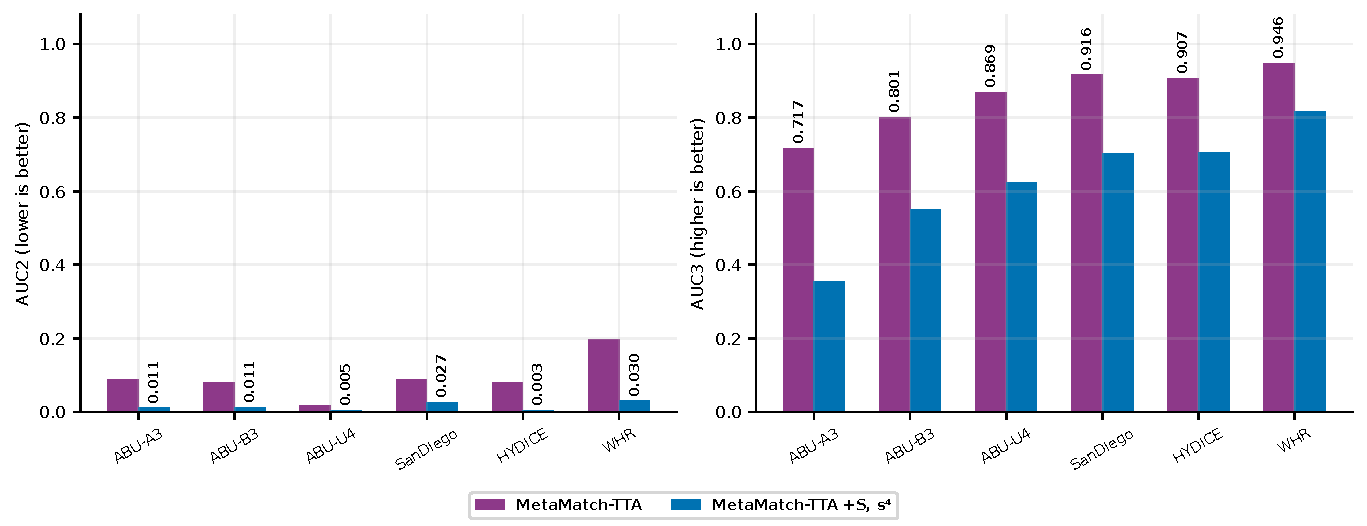
\includegraphics[width=1.0\linewidth]{recent_only_figures/fig_sharp.pdf}\caption{Threshold-integral metrics of two outputs under P1, comparing \method{} with \method{} +S after an $s^4$ transformation. Lower AUC$_2$ and higher AUC$_3$ are preferred. The better value for each scene is bold. The outputs differ in both model stage and score transformation.}\label{full:fig:sharp}\end{figure}

Figure~\ref{full:fig:sharp} compares integrated false-alarm and target responses for two output configurations. On ABU-U4, \method{} has AUC$_2$ and AUC$_3$ values of 0.0174 and 0.8689. After student fusion and the $s^4$ transformation, these become 0.0048 and 0.6226. The transformed output combines a lower background response with compressed target responses, while the two configurations retain ROC-AUC values of 0.9970 and 0.9972. High ranking accuracy is already present in the original matching output. For the same score vector, a strictly monotonic fourth-power transformation preserves ranking and adjusts the output distribution.

\subsection{Task Learning and Spectral Pooling}

\begin{figure}[H]\centering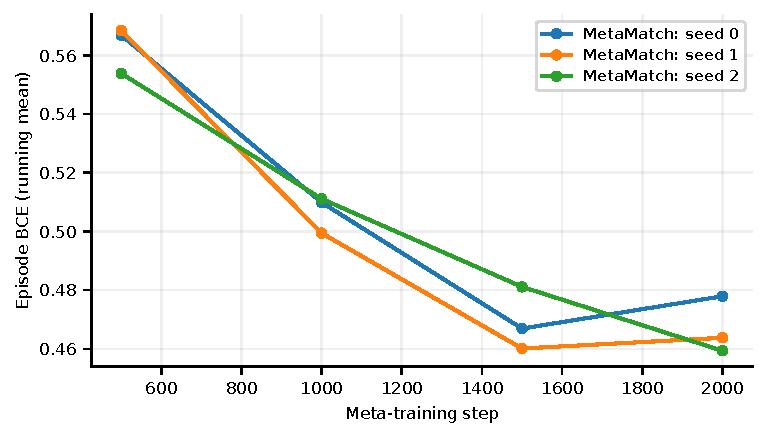
\includegraphics[width=0.65\linewidth]{full_figures/fig_training.pdf}\caption{Task BCE trajectories of \textbf{\matcher{}} for training seeds 0, 1, and 2. Running means are recorded every 500 steps. The curves describe optimization on development tasks. Detection performance on target scenes is evaluated separately.}\label{full:fig:training}\end{figure}

Figure~\ref{full:fig:training} shows material-pair optimization from three training initializations. Task BCE decreases from approximately 0.55--0.57 at step 500 to 0.46--0.48 at step 2,000, with a consistent downward trend across seeds. Each task changes the target material, reference construction, and query observations. Reducing the loss therefore requires relationships reusable across samples, and memorizing a fixed reference cannot satisfy the objective. The trajectories indicate that the shared encoder learns to distinguish positive and negative material pairs amid these changes. Seed-specific target-scene results then test whether this capability transfers to new images. Together, they support learning a stable shared matching function through material tasks.

\begin{figure}[H]\centering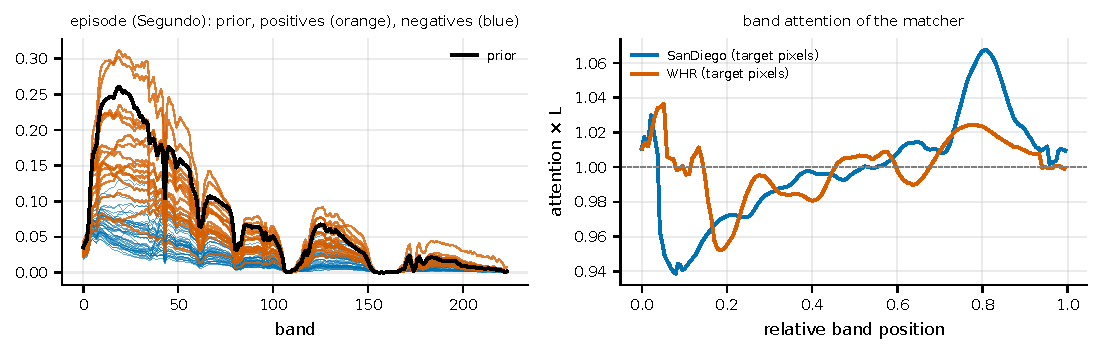
\includegraphics[width=1.0\linewidth]{full_figures/fig_episode_att.pdf}\caption{A material-task example from Segundo (left) and spectral attention on SanDiego and WHR (right). Orange and blue denote positive and negative queries, respectively, and black denotes the reference. Attention weights are multiplied by the band count $L$, so the dashed line at 1 represents uniform pooling.}\label{full:fig:episode}\end{figure}

Figure~\ref{full:fig:episode} connects task construction with spectral pooling. Positive queries on Segundo resemble the reference in spectral shape but differ noticeably in amplitude, requiring \matcher{} to preserve material consistency despite observation differences. Attention on SanDiego and WHR adjusts around uniform weighting with different magnitudes. SanDiego places greater weight near relative band position 0.8, while the WHR distribution is flatter. The network therefore uses the full spectrum with moderate reweighting, without concentrating on a single band in these examples. Attention-weighted means, ordinary means, and maxima jointly form a fixed-length representation that connects variable-length inputs to the same prediction head. This visualization explains how material-variation tasks interact with sequence pooling and provides a structural interpretation of variable-length spectral processing with shared parameters.

\FloatBarrier

\section{Discussion}
The experiments identify reduced reference-information requirements and reuse of learned material relationships as the principal benefits of the design. The single-pixel macro-average ROC-AUC is 0.9902, and the five-pixel reference matches the complete-mean result of 0.9924 at the reported precision. A small number of target observations can therefore drive accurate image-wide ranking. Ablations of spectral augmentation and whitened channels reveal the benefits of tolerating observation changes and incorporating background differences. The complete refined model obtains the highest ROC-AUC in 11 of 12 comparisons. ROC curves, detection maps, and score distributions connect these numerical results to high responses at dispersed targets and low responses over most background pixels. Limited-reference performance, component comparisons, and pixel-level evidence jointly support background-conditioned material matching.

Gradient-free reference updates use this pairing capability to collect additional observations from the current image. On HYDICE, the single-pixel result combines a higher mean with lower variability across runs, showing that adaptation can be achieved by improving the reference. On ABU-B3, the candidate count exceeds the ground-truth target count, explicitly identifying a source of background contamination in the mean. The P1 and P4 stage comparisons show that the benefit of reference updates depends on the relationship between the initial description and candidate information. This suggests prioritizing material consistency in candidate selection and then using multiple observations to reduce sensitivity to an individual reference. The fixed-network pairing interface allows such improvements to focus on reference selection while preserving discrimination learned across scenes.

The method combines knowledge learned across scenes with current-image statistics in a network of 0.1659 M parameters. Material-cluster tasks and labeled tasks sampled with probability 0.2 jointly train the matcher, while sequence pooling connects different band counts to a shared prediction head. With mean references, the macro-average ROC-AUC values of \method{} and FAME-Net are 0.9924 and 0.9982, respectively, showing the high accuracy of detection tailored to sufficiently informative references. The advantage demonstrated here concerns unified processing of single-pixel, few-pixel mean, and prescribed perturbed references with the same fixed-weight model. Invoking existing material relationships through changes in the reference and background conditions offers a practical way to reduce model adaptation for new images.



\section{Conclusion}
This paper presents \method{}, a background-conditioned pairwise matching method that combines raw spectral relationships, whitened spectral relationships, and analytical statistics for material discrimination. Reference randomization and spectral augmentation train a shared matching function. Across six target scenes, macro-average ROC-AUC reaches 0.9902 with single-pixel references and 0.9903 with synthetically perturbed references. Five-pixel references match the complete-mean accuracy of 0.9924 at the reported precision, demonstrating effective use of limited target observations. Component experiments support the discrimination benefits of background conditioning and spectral augmentation. Stage comparisons show that direct matching establishes most detection capability, while scene candidates can supplement individual observations. ROC curves, spatial responses, and score distributions provide corresponding evidence of target detection and background separation. Fixed network weights, variable-length spectral pooling, and gradient-free reference updates enable reuse across images, providing a compact implementation for hyperspectral target detection with limited reference information.

\clearpage
\begingroup\footnotesize
\begin{thebibliography}{99}
\setlength{\itemsep}{1pt}
\bibitem{mlsn} Y. Wang, X. Chen, F. Wang, M. Song, and C. Yu, ``Meta-Learning Based Hyperspectral Target Detection Using Siamese Network,'' \emph{IEEE Transactions on Geoscience and Remote Sensing}, vol. 60, art. 5527913, 2022, pp. 1--13. \href{https://doi.org/10.1109/TGRS.2022.3169970}{doi: 10.1109/TGRS.2022.3169970}.
\bibitem{htdmamba} D. Shen, X. Zhu, J. Tian, J. Liu, Z. Du, H. Wang, and X. Ma, ``HTD-Mamba: Efficient Hyperspectral Target Detection With Pyramid State Space Model,'' \emph{IEEE Transactions on Geoscience and Remote Sensing}, vol. 63, pp. 1--15, 2025. \href{https://doi.org/10.1109/TGRS.2025.3547019}{doi: 10.1109/TGRS.2025.3547019}.
\bibitem{pstd} X. Han, Y. Wei, H. Zhang, Q. Xu, and W. Sun, ``Tuning to Real for Single-Spectrum Hyperspectral Target Detection,'' in \emph{Proc. 13th Workshop on Hyperspectral Imaging and Signal Processing: Evolution in Remote Sensing (WHISPERS)}, 2023, pp. 1--5. \href{https://doi.org/10.1109/WHISPERS61460.2023.10430857}{doi: 10.1109/WHISPERS61460.2023.10430857}.
\bibitem{tasr} R. Gerster and P. St\"utz, ``Towards Robust Hyperspectral Target Detection via Test-Time Spectrum Adaptation,'' \emph{Remote Sensing}, vol. 17, no. 16, art. 2756, 2025. \href{https://doi.org/10.3390/rs17162756}{doi: 10.3390/rs17162756}.
\bibitem{fame} Z. Yang, M. Zhang, J. Wang, Y. Gao, W. Liao, and W. Li, ``A Dual-Network Framework With Adversarial GMM Augmentation and Frequency-Mamba Fusion for Hyperspectral Target Detection,'' \emph{IEEE Transactions on Neural Networks and Learning Systems}, vol. 37, no. 10, pp. 5090--5104, 2026. \href{https://doi.org/10.1109/TNNLS.2026.3682921}{doi: 10.1109/TNNLS.2026.3682921}.
\bibitem{selfmtl} F. Luo, S. Shi, K. Qin, T. Guo, C. Fu, and Z. Lin, ``SelfMTL: Self-Supervised Meta-Transfer Learning via Contrastive Representation for Hyperspectral Target Detection,'' \emph{IEEE Transactions on Geoscience and Remote Sensing}, vol. 63, art. 5508613, 2025, pp. 1--13. \href{https://doi.org/10.1109/TGRS.2025.3550283}{doi: 10.1109/TGRS.2025.3550283}.
\bibitem{clhtd} X. Chen, Y. Wang, Z. Che, L. Zhu, M. Song, and H. Yu, ``Contrastive Learning for Hyperspectral Target Detection,'' in \emph{Proc. IEEE International Geoscience and Remote Sensing Symposium (IGARSS)}, 2022, pp. 887--890. \href{https://doi.org/10.1109/IGARSS46834.2022.9883439}{doi: 10.1109/IGARSS46834.2022.9883439}.
\bibitem{specmamba} L. Gong, Q. Xie, Y. Chen, Z. Chen, F. Fan, S. Zhao, and C. Li, ``Physics-Aligned Spectral Mamba: Decoupling Semantics and Dynamics for Few-Shot Hyperspectral Target Detection,'' arXiv:2604.05562, 2026 (preprint). \url{https://arxiv.org/abs/2604.05562}.
\bibitem{hyperfree} J. Li \emph{et al.}, ``HyperFree: A Channel-adaptive and Tuning-free Foundation Model for Hyperspectral Remote Sensing Imagery,'' in \emph{Proc. IEEE/CVF Conference on Computer Vision and Pattern Recognition (CVPR)}, 2025, pp. 23048--23058. \href{https://openaccess.thecvf.com/content/CVPR2025/html/Li_HyperFree_A_Channel-adaptive_and_Tuning-free_Foundation_Model_for_Hyperspectral_Remote_CVPR_2025_paper.html}{Official CVF paper page}.
\bibitem{htmnet2025} X. Zheng, Y. Kuang, Y. Huo, W. Zhu, M. Zhang, and H. Wang, ``HTMNet: Hybrid Transformer--Mamba Network for Hyperspectral Target Detection,'' \emph{Remote Sensing}, vol. 17, no. 17, art. 3015, 2025. \href{https://doi.org/10.3390/rs17173015}{doi: 10.3390/rs17173015}.
\bibitem{sage2025} T. Li, H. Jin, and Z. Li, ``Hyperspectral target detection based on graph sampling and aggregation network,'' \emph{PLOS ONE}, vol. 20, no. 4, art. e0320043, 2025. \href{https://doi.org/10.1371/journal.pone.0320043}{doi: 10.1371/journal.pone.0320043}.
\bibitem{spwcg2026} Z. Mao, C. Feng, S. Liu, Y. Huang, and D. Wu, ``Diffusion-Enhanced Hyperspectral Target Detection with Spectral Similarity Purification and Wavelet Cross-Gating,'' \emph{Applied Sciences}, vol. 16, no. 20, art. 10129, 2026. \href{https://doi.org/10.3390/app162010129}{doi: 10.3390/app162010129}.
\bibitem{rsmf2026} B. Asghari Beirami, ``Spectral matched filter ensembles for hyperspectral target detection,'' \emph{Revista de Teledetecci\'on}, no. 68, art. e26360, 2026. \href{https://doi.org/10.4995/raet.2026.26360}{doi: 10.4995/raet.2026.26360}.
\bibitem{amf} F. C. Robey, D. R. Fuhrmann, E. J. Kelly, and R. Nitzberg, ``A CFAR adaptive matched filter detector,'' \emph{IEEE Transactions on Aerospace and Electronic Systems}, vol. 28, no. 1, pp. 208--216, 1992. \href{https://doi.org/10.1109/7.135446}{doi: 10.1109/7.135446}.
\bibitem{ace} S. Kraut and L. L. Scharf, ``The CFAR adaptive subspace detector is a scale-invariant GLRT,'' \emph{IEEE Transactions on Signal Processing}, vol. 47, no. 9, pp. 2538--2541, 1999. \href{https://doi.org/10.1109/78.782198}{doi: 10.1109/78.782198}.
\bibitem{chang2021} C.-I. Chang, ``An effective evaluation tool for hyperspectral target detection: 3D receiver operating characteristic curve analysis,'' \emph{IEEE Trans. Geosci. Remote Sens.}, vol. 59, no. 6, pp. 5131--5153, 2021.
\bibitem{gdpncl2025} J. Wu, R. Liu, and N. Wang, ``Contrastive Learning-Based Hyperspectral Image Target Detection Using a Gated Dual-Path Network,'' \emph{Remote Sensing}, vol. 17, no. 14, art. 2345, 2025. \href{https://doi.org/10.3390/rs17142345}{doi: 10.3390/rs17142345}.
\bibitem{dsml2025} Y. Wang, C. Deng, H. Wang, E. Zhao, and Q. Lan, ``Deep spectral metric learning with Siamese network for hyperspectral target detection,'' \emph{Infrared Physics \& Technology}, vol. 150, art. 106056, 2025. \href{https://doi.org/10.1016/j.infrared.2025.106056}{doi: 10.1016/j.infrared.2025.106056}.
\bibitem{htdda2025} Z. Zhuang, J. Lan, and Y. Zeng, ``Hyperspectral Target Detection Based on Masked Autoencoder Data Augmentation,'' \emph{Remote Sensing}, vol. 17, no. 6, art. 1097, 2025. \href{https://doi.org/10.3390/rs17061097}{doi: 10.3390/rs17061097}.
\bibitem{bastnet2025} Z. Wang, K. Tan, X. Wang, and X. Xu, ``Hyperspectral Target Detection Based on a Background-Aware Sparse Transformer Network,'' \emph{IEEE Transactions on Geoscience and Remote Sensing}, vol. 63, art. 5525219, pp. 1--19, 2025. \href{https://doi.org/10.1109/TGRS.2025.3608271}{doi: 10.1109/TGRS.2025.3608271}.
\bibitem{siddn2025} J. Gong, Z. Huang, Z. Yang, X. Ding, and F. Li, ``Spectral Information Divergence-Driven Diffusion Networks for Hyperspectral Target Detection,'' \emph{Applied Sciences}, vol. 15, no. 8, art. 4076, 2025. \href{https://doi.org/10.3390/app15084076}{doi: 10.3390/app15084076}.
\bibitem{sdgat2026} M. Wang, Y. Pang, and Y. Xiao, ``Superpixel-driven graph adaptive transformer for hyperspectral target detection,'' \emph{Infrared Physics \& Technology}, vol. 156, art. 106557, 2026. \href{https://doi.org/10.1016/j.infrared.2026.106557}{doi: 10.1016/j.infrared.2026.106557}.
\bibitem{wtgssl2025} H. Qin, S. Wang, Y. Li, W. Xie, K. Jiang, and K. Cao, ``Hyperspectral Target Detection Based on Generative Self-Supervised Learning With Wavelet Transform,'' \emph{IEEE Transactions on Geoscience and Remote Sensing}, vol. 63, art. 5510815, pp. 1--15, 2025. \href{https://doi.org/10.1109/TGRS.2025.3549771}{doi: 10.1109/TGRS.2025.3549771}.
\bibitem{htdgmd2026} S. Wang, H. Qin, J. Ling, Z. Ye, Y. Qiu, G. Chen, J. Ma, W. Xie, and Y. Li, ``HTD-GMD: Hyperspectral Target Detection Based on Generative Self-supervised Learning with Mamba and Diffusion Models,'' \emph{IEEE Transactions on Circuits and Systems for Video Technology}, early access, Aug. 20, 2026. \href{https://doi.org/10.1109/TCSVT.2026.3725281}{doi: 10.1109/TCSVT.2026.3725281}.
\bibitem{ueml2026} Q. Liu, Y. Xu, Z. Wu, J. Peng, and Z. Wei, ``Unbalanced episode meta-learning with Bi-Sparse contrastive network for hyperspectral target detection,'' \emph{Pattern Recognition}, vol. 170, art. 112030, 2026. \href{https://doi.org/10.1016/j.patcog.2025.112030}{doi: 10.1016/j.patcog.2025.112030}.
\bibitem{uclkd2025} F. Mo, Z. Li, X. Gong, C. Wang, and B. Yuan, ``Hyperspectral Target Detection Based on Unsupervised Contrastive Learning and Spatial--Spectral Knowledge Distillation,'' \emph{IEEE Geoscience and Remote Sensing Letters}, vol. 22, art. 5504605, pp. 1--5, 2025. \href{https://doi.org/10.1109/LGRS.2025.3566955}{doi: 10.1109/LGRS.2025.3566955}.
\bibitem{ssbdm2026} D. Shen, W. Kong, X. Xiao, J. Liu, Z. Du, X. Ma, W. Zhao, and H. Wang, ``SSBDM: A Spectral--Spatial Bilinear Decomposition Model With Adaptive Multikernel Dictionary for Hyperspectral Target Detection,'' \emph{IEEE Journal of Selected Topics in Applied Earth Observations and Remote Sensing}, vol. 19, pp. 9347--9365, 2026. \href{https://doi.org/10.1109/JSTARS.2026.3670876}{doi: 10.1109/JSTARS.2026.3670876}.
\bibitem{huclnet2025} J. Qi, X. Liu, and P. Zhong, ``Empowering Hybrid-Level Contrastive Learning for Hyperspectral Underwater Target Detection in Nearshore Environment,'' \emph{IEEE Transactions on Geoscience and Remote Sensing}, vol. 63, art. 5526717, pp. 1--17, 2025. \href{https://doi.org/10.1109/TGRS.2025.3613208}{doi: 10.1109/TGRS.2025.3613208}.
\end{thebibliography}
\endgroup

\end{document}
